\Opensolutionfile{ans}[ans/ansCD2D3-2.0]
\section{TÍCH PHÂN – CÁC PHƯƠNG PHÁP TÍNH TÍCH PHÂN}
\subsection{KIẾN THỨC CƠ BẢN}
\subsubsection{Định nghĩa} Cho hàm số $f$ liên tục trên khoảng $K$ và $a,b$ là hai số bất kì thuộc $K$. Nếu $F$ là một nguyên hàm của $f$ trên $K$ thì hiệu số $F(b)-F(a)$ được gọi là tích phân của hàm số $f$ từ $a$ đến $b$ và kí hiệu là $\displaystyle\int\limits_a^b f(x)\mathrm{\,d}x$.\\
Ta gọi: $a$ là cận dưới, $b$ là cận trên, $f$ là hàm số dưới dấu tích phân, $f(x)\mathrm{\,d}x$ là biểu thức dưới dấu tích phân, $x$ biến số lấy tích phân.\\
Nhận xét:\\
a) Nếu $a<b$ thì ta gọi $\displaystyle\int\limits_a^b f(x)\mathrm{\,d}x$ là tích phân của $f$ trên đoạn $[a;b]$.\\
b) Hiệu số $F(b)-F(a)$ còn được kí hiệu là $F(x)\bigg|_a^b$. Khi đó: $\displaystyle\int\limits_a^b f(x)\mathrm{\,d}x=F(x)\bigg|_a^b=F(b)-F(a)$.\\
c) Tích phân \textbf{không} phụ thuộc biến số (điều này sẽ mang lại lợi ích cho ta để tính một số tích phân đặc biệt), tức là $\displaystyle\int\limits_a^b f(x)\mathrm{\,d}x=\displaystyle\int\limits_a^b f(t)\mathrm{\,d}t=\displaystyle\int\limits_a^b f(u)\mathrm{\,d}u=\cdots =F(b)-F(a)$.\\
\subsubsection{Tính chất} Cho $k$ là hằng số.\\
\begin{listEX}[2]
\item $\displaystyle\int\limits_a^a f(x)\mathrm{\,d}x=0$ 
\item $\displaystyle\int\limits_a^b f(x)\mathrm{\,d}x=-\displaystyle\int\limits_b^a f(x)\mathrm{\,d}x$
\item $\displaystyle\int\limits_a^b k\cdot f(x)\mathrm{\,d}x=k\displaystyle\int\limits_a^b f(x)\mathrm{\,d}x$ 
\item $\displaystyle\int\limits_a^b[f(x)+g(x)]\mathrm{\,d}x=\displaystyle\int\limits_a^b f(x)\mathrm{\,d}x+\displaystyle\int\limits_a^b g(x)\mathrm{\,d}x$
\item Tính chất chèn cận:\\
$\displaystyle\int\limits_a^b f(x)\mathrm{\,d}x=\displaystyle\int\limits_a^c f(x)\mathrm{\,d}x+\displaystyle\int\limits_c^b f(x)\mathrm{\,d}x$ 
\end{listEX}
\subsection{CÁC DẠNG TOÁN}
\begin{dang}{SỬ DỤNG ĐỊNH NGHĨA TÍCH PHÂN}
\end{dang}
\begin{ex}%[2D3Y2-1]%Câu 1.
	Tính các tích phân sau:
		\begin{enumerate}
		\begin{multicols}{2}
		\item $I=\displaystyle\int\limits_0^1 3x^2\mathrm{\,d}x$
		\item $I=\displaystyle\int\limits_1^4\dfrac{1}{\sqrt{x}}\mathrm{\,d}x$
		\item $I=\displaystyle\int\limits_0^{\ln 2} 2^x\mathrm{\,d}x$.
		\item $I=\displaystyle\int\limits_0^{\tfrac{\pi}{4}}\sin x\mathrm{\,d}x$.
			\end{multicols}
		\end{enumerate}
	\loigiai{
		\begin{enumEX}{1}
			\item $I=\displaystyle\int\limits_0^1 3x^2\mathrm{\,d}x= x^3\bigg|_0^1=1-0=1$.
			\item $I=\displaystyle\int\limits_1^4\dfrac{1}{\sqrt{x}}\mathrm{\,d}x= 2\sqrt{x}\bigg|_1^4=2(2-1)=2$.
			\item $I=\displaystyle\int\limits_0^1 2^x\mathrm{\,d}x=\dfrac{2^x}{\ln 2}\bigg|_0^1=\dfrac{1}{\ln 2}\left(2^1-2^0\right)=\dfrac{1}{\ln 2}$.
			\item $I=\displaystyle\int\limits_0^{\tfrac{\pi}{4}}\sin x\mathrm{\,d}x= -\cos x\bigg|_0^{\tfrac{\pi}{4}}=-\left(\dfrac{1}{\sqrt{2}}-1\right)=1-\dfrac{1}{\sqrt{2}}$.
		\end{enumEX}	
	}
\end{ex}
\begin{ex}%[2D3B2-1]%Câu 2.
	Gọi $F(x)$ là nguyên hàm của hàm số $f(x)=\mathrm{e}^x$. Tính $F(2\ln 2)-F(\ln 2)$.
	\loigiai{
		Vì hàm số $f(x)=\mathrm{e}^x$ liên tục trên đoạn $\left[\ln 2;2\ln 2\right]$ nên ta có:\\
		$F(\ln 4)-F(\ln 2)=\displaystyle\int\limits_{\ln 2}^{\ln 4} f(x)\mathrm{\,d}x=\displaystyle\int\limits_{\ln 2}^{\ln 4}\mathrm{e}^x\mathrm{\,d}x=\mathrm{e}^x\bigg|_{\ln 2}^{\ln 4}=2$.}
\end{ex}
\begin{ex}%[2D3B2-1]%Câu 3.
	Gọi $F(x)$ là nguyên hàm của hàm số $f(x)=\dfrac{1}{x}$ thỏa điều kiện $F(1)=2$. Tính $F(e)$.
	\loigiai{
		Vì hàm số $f(x)=\dfrac{1}{x}$ liên tục trên đoạn $[1;e]$ nên ta có:\\
		$F(e)-F(1)=\displaystyle\int\limits_1^e f(x)\mathrm{\,d}x=\displaystyle\int\limits_1^e\dfrac{1}{x}\mathrm{\,d}x=\ln |x|\bigg|_1^e=1$.\\
		Suy ra: $F(e)=1+F(1)=1+2=3$.}
\end{ex}
\begin{ex}%[2D3B2-1]%Câu 4.
	Chứng minh $F(x)=\ln \left(x+\sqrt{x^2+1}\right)$ là một nguyên hàm của hàm số $f(x)=\dfrac{1}{\sqrt{x^2+1}}$. Từ đó tính tích phân $I=\displaystyle\int\limits_0^1\dfrac{1}{\sqrt{x^2+1}}\mathrm{\,d}x$.
	\loigiai{
		Ta có:\\
		$F’(x)=\dfrac{\left(x+\sqrt{x^2+1}\right)’}{x+\sqrt{x^2+1}}=\dfrac{1+\dfrac{x}{\sqrt{x^2+1}}}{x+\sqrt{x^2+1}}=\dfrac{1}{\sqrt{x^2+1}}=f(x)$.\\
		Do đó:\\
		$I=\displaystyle\int\limits_0^1\dfrac{1}{\sqrt{x^2+1}}\mathrm{\,d}x=\ln \left(x+\sqrt{x^2+1}\right)\bigg|_0^1=\ln (1+\sqrt{2})$.}
\end{ex}
\begin{ex}%[2D3B2-1]%Câu 5.
	Chứng minh $F(x)=\dfrac{1}{ad-bc}\ln \left|\dfrac{ax+b}{cx+d}\right|$ là một nguyên hàm của hàm số $f(x)=\dfrac{1}{(ax+b)(cx+d)}$. Từ đó tính tích phân $I=\displaystyle\int\limits_0^1\dfrac{1}{(2x+1)(x+1)}\mathrm{\,d}x$.
	\loigiai{
		Ta có:\\
		$F’(x)=\dfrac{1}{ad-bc}\left(\ln |ax+b|-\ln |cx+d|\right)’=\dfrac{1}{ad-bc}\left(\dfrac{a}{ax+b}-\dfrac{c}{cx+d}\right)=\dfrac{1}{(ax+b)(cx+d)}=f(x)$.\\
		Do đó:\\
		$I=\displaystyle\int\limits_0^1\dfrac{1}{(2x+1)(x+1)}\mathrm{\,d}x=\dfrac{1}{2-1}\ln \left|\dfrac{2x+1}{x+1}\right|\bigg|_0^1=\ln \dfrac{3}{2}-\ln 1=\ln \dfrac{3}{2}$.}
\end{ex}
\begin{dang}{SỬ DỤNG TÍNH CHẤT TÍCH PHÂN.}
\end{dang}
\begin{ex}%[2D3Y2-1]%Câu 6.
	Tính các tích phân sau:
\begin{listEX}[3]
	\item $I=\displaystyle\int\limits_0^1\left(4x^3-\mathrm{e}^x\right)\mathrm{\,d}x$
	\item $I=\displaystyle\int\limits_1^2\left(3^x-\dfrac{1}{x}\right)\mathrm{\,d}x$
	\item $I=\displaystyle\int\limits_0^{\pi}\left(\sin x+2\cos x\right)\mathrm{\,d}x$.
\end{listEX}
	\loigiai{
		\begin{enumerate}[a)]
			\item $I=\displaystyle\int\limits_0^1\left(4x^3-\mathrm{e}^x\right)\mathrm{\,d}x= x^4\bigg|_0^1-\mathrm{e}^x\bigg|_0^1=1-(e-1)=2-e$. \item $ I=\displaystyle\int\limits_1^2\left(3^x-\dfrac{1}{x}\right)\mathrm{\,d}x=\dfrac{3^x}{\ln 3}\bigg|_1^2-\ln |x|\bigg|_1^2=\dfrac{1}{\ln 3}(9-3)-\ln 2=\dfrac{6}{\ln 3}-\ln 2$.
			\item $I=\displaystyle\int\limits_0^{\pi}\left(\sin x+2\cos x\right)\mathrm{\,d}x= -\cos x\bigg|_0^{\pi}+ 2\sin x\bigg|_0^{\pi}=2$.
	\end{enumerate}}
\end{ex}
\begin{ex}%[2D3B2-1]%Câu 7.
	Tính $I=\displaystyle\int\limits_1^2\mathrm{e}^x\ln x\mathrm{\,d}x+\displaystyle\int\limits_1^2\mathrm{e}^t(1-\ln t)\mathrm{\,d}t$.
	\loigiai{
		$I=\displaystyle\int\limits_1^2\mathrm{e}^x\ln x\mathrm{\,d}x+\displaystyle\int\limits_1^2\mathrm{e}^x(1-\ln x)\mathrm{\,d}x=\displaystyle\int\limits_1^2\mathrm{e}^x\mathrm{\,d}x=\mathrm{e}^2-e$.}
\end{ex}
\begin{ex}%[2D3B2-1]%Câu 8.
	Tính $I=\displaystyle\int\limits_{\tfrac{\pi}{2}}^{\pi}\sin\dfrac{t}{2}\ln t\mathrm{\,d}t+\displaystyle\int\limits_{\pi}^{\tfrac{\pi}{2}}\sin\dfrac{u}{2}\left(ln u-\sin\dfrac{u}{2}\right)\mathrm{\,d}u$.
	\loigiai{
		$I=\displaystyle\int\limits_{\tfrac{\pi}{2}}^{\pi}\sin\dfrac{x}{2}\ln x\mathrm{\,d}x-\displaystyle\int\limits_{\tfrac{\pi}{2}}^{\pi}\sin\dfrac{x}{2}\left(\ln x-\sin\dfrac{x}{2}\right)\mathrm{\,d}x$.\\
		$=\displaystyle\int\limits_{\tfrac{\pi}{2}}^{\pi}\sin^2\dfrac{x}{2}\mathrm{\,d}x=\displaystyle\int\limits_{\tfrac{\pi}{2}}^{\pi}\dfrac{1-\cos x}{2}\mathrm{\,d}x=\dfrac{1}{2}x\bigg|_{\tfrac{\pi}{2}}^{\pi}-\dfrac{1}{2}\sin x\bigg|_{\tfrac{\pi}{2}}^{\pi}=\dfrac{\pi}{4}+\dfrac{1}{2}$.}
\end{ex}
\begin{dang}{SỬ DỤNG TÍNH CHẤT CHÈN CẬN ĐỂ TÍNH TÍCH PHÂN}
\textbf{Tích phân của hàm chứa dấu trị tuyệt đối.}
	a) Yêu cầu: Tính tích phân $I=\displaystyle\int\limits_a^b|f(x)|\mathrm{\,d}x$.\\
	b) Phương pháp:\\
	+ Bước 1: Xét dấu của $f(x)$ trên khoảng $(a;b)$.\\
	-Giải phương trình $f(x)=0\Leftrightarrow x=x_i\in(a;b)$.\\
	-Lập bảng xét dấu của $f(x)$ trên khoảng $(a;b)$.\\
	+ Bước 2: Chèn cận $x_i$ và đồng thời bỏ dấu gttđ (căn cứ vào BXD) ta được các tích phân cơ bản.\\
	$I=\displaystyle\int\limits_a^b\left|f(x)\right|\mathrm{\,d}x=\displaystyle\int\limits_a^{x_i}\left|f(x)\right|\mathrm{\,d}x+\displaystyle\int\limits_{x_i}^b\left|f(x)\right|\mathrm{\,d}x$.\\
	Chú ý: Nếu $f(x)$ không đổi dấu trên đoạn $[a;b]$ thì $I=\displaystyle\int\limits_a^b\left|f(x)\right|\mathrm{\,d}x=\left|\displaystyle\int\limits_a^b f(x)\mathrm{\,d}x\right|$.
\end{dang}
\begin{ex}%[2D3B2-1]%Câu 9.
	Tính các tích phân:
\begin{listEX}[2]
	\item $I=\displaystyle\int\limits_0^2|x-1|\mathrm{\,d}x$
	\item $I=\displaystyle\int\limits_0^3\left|x^2-x\right|\mathrm{\,d}x$
	\item $I=\displaystyle\int\limits_{-4}^2\left|x^2+2x-3\right|\mathrm{\,d}x$
	\item $I=\displaystyle\int\limits_{-2}^2\left|2x-|x+1|\right|\mathrm{\,d}x$.
\end{listEX}
	\loigiai{
		a) $ I=\displaystyle\int\limits_0^2|x-1|\mathrm{\,d}x= \displaystyle\int\limits_0^1|x-1|\mathrm{\,d}x+\displaystyle\int\limits_1^2|x-1|\mathrm{\,d}x=-\displaystyle\int\limits_0^1(x-1)\mathrm{\,d}x+\displaystyle\int\limits_1^2(x-1)\mathrm{\,d}x=\dfrac{1}{2}+\dfrac{1}{2}=1$.\\
		b) Xét trên khoảng $(0;3)$ ta có: $x^2-x=0\Leftrightarrow\hoac{&x=0(l)\\&x=1.}$ \\
		Bảng xét dấu: 
		\begin{center}
			\begin{tikzpicture}
		\tkzTabInit[deltacl=0.5,espcl=2.5,lgt=2]
		{$x$/1,$x^2-x$/1}
		{$0$,$1$,$3$}
		\tkzTabLine{,-,0,+,}
		\end{tikzpicture}
		\end{center}
		Suy ra:\\
		$I=-\displaystyle\int\limits_0^1\left(x^2-x\right)\mathrm{\,d}x+\displaystyle\int\limits_1^3\left(x^2-x\right)\mathrm{\,d}x=\dfrac{1}{6}+\dfrac{14}{3}=\dfrac{29}{6}$.\\
		c) Xét trên khoảng $(-2;2)$ ta có: $x^2+2x-3=0\Leftrightarrow\hoac{&x=-3\\&x=1.}$ \\
		Bảng xét dấu: 
		\begin{center}
			\begin{tikzpicture}
		\tkzTabInit[deltacl=0.5,espcl=2.5,lgt=3]
		{$x$/1,$x^2+2x-3$/1}
		{$-4$,$-3$,$1$,$2$}
		\tkzTabLine{,+,0,-,0,+}
		\end{tikzpicture}
		\end{center}
		Suy ra:\\
		$I=\displaystyle\int\limits_{-4}^{-3}\left(x^2+2x-3\right)\mathrm{\,d}x-\displaystyle\int\limits_{-3}^1\left(x^2+2x-3\right)\mathrm{\,d}x+\displaystyle\int\limits_1^2\left(x^2+2x-3\right)\mathrm{\,d}x=\dfrac{7}{3}+\dfrac{32}{3}+\dfrac{7}{3}=\dfrac{46}{3}$.\\
		d) Xét trên khoảng $(-2;2)$ ta có: $x+1=0\Leftrightarrow x=-1$.\\
		Bảng xét dấu: 
		\begin{center}
			\begin{tikzpicture}
			\tkzTabInit[deltacl=0.5,espcl=2.5,lgt=2]
			{$x$/1,$x+1$/1}
			{$-2$,$-1$,$2$}
			\tkzTabLine{,-,0,+,}
			\end{tikzpicture}
		\end{center}
		Suy ra:\\
		$I=\displaystyle\int\limits_{-2}^1|2x+x+1|\mathrm{\,d}x+\displaystyle\int\limits_1^2|2x-x-1|\mathrm{\,d}x=\displaystyle\int\limits_{-2}^1|3x+1|\mathrm{\,d}x+\displaystyle\int\limits_1^2|x-1|\mathrm{\,d}x=I_1+I_2$.\\
		Ta có:\\
		$I_1=\displaystyle\int\limits_{-2}^1|3x+1|\mathrm{\,d}x=-\displaystyle\int\limits_{-2}^{-\tfrac{1}{3}}(3x+1)\mathrm{\,d}x+\displaystyle\int\limits_{-\tfrac{1}{3}}^1(3x+1)\mathrm{\,d}x=\dfrac{41}{6}$.\\
		$I_2=\displaystyle\int\limits_1^2|x-1|\mathrm{\,d}x=\displaystyle\int\limits_1^2(x-1)\mathrm{\,d}x=\dfrac{1}{2}$.\\
		Vậy: $I=\dfrac{41}{6}+\dfrac{1}{2}=\dfrac{22}{3}$.}
\end{ex}
\begin{ex}%[2D3B2-1]%Câu 10.
	Tính $I=\displaystyle\int\limits_0^{\pi}\sqrt{1-\cos 2x}\mathrm{\,d}x$.
	\loigiai{
		$I=\displaystyle\int\limits_0^{\pi}\sqrt{\dfrac{1+\cos 2x}{2}}\mathrm{\,d}x=\displaystyle\int\limits_0^{\pi}\sqrt{\cos^2x}\mathrm{\,d}x=\displaystyle\int\limits_0^{\pi}|\cos x|\mathrm{\,d}x=\displaystyle\int\limits_0^{\tfrac{\pi}{2}}\cos x\mathrm{\,d}x-\displaystyle\int\limits_{\tfrac{\pi}{2}}^{\pi}\cos x\mathrm{\,d}x=1+1=2$.}
\end{ex}
\begin{ex}%[2D3B2-1]%Câu 11.
	Tính $I=\displaystyle\int\limits_0^{\tfrac{\pi}{2}}\sqrt{\dfrac{1-\sin 2x}{2}}\mathrm{\,d}x$.
	\loigiai{
		Ta có:\\
		$I=\displaystyle\int\limits_0^{\tfrac{\pi}{2}}\sqrt{\dfrac{1-\cos\left(\dfrac{\pi}{2}-2x\right)}{2}}\mathrm{\,d}x=\displaystyle\int\limits_0^{\tfrac{\pi}{2}}\sqrt{\sin^2\left(\dfrac{\pi}{4}-x\right)}\mathrm{\,d}x=\displaystyle\int\limits_0^{\tfrac{\pi}{2}}\left|\sin\left(x-\dfrac{\pi}{4}\right)\right|\mathrm{\,d}x$.\\
		Xét trên khoảng $\left(0;\dfrac{\pi}{2}\right)$, ta có: $\sin\left(x-\dfrac{\pi}{4}\right)=0\Leftrightarrow x=\dfrac{\pi}{4}$.\\
		Bảng xét dấu: 
		\begin{center}
			\begin{tikzpicture}
			\tkzTabInit[deltacl=0.5,espcl=2.5,lgt=3]
			{$x$/1,$\sin\left(x-\dfrac{\pi}{4}\right)$/1}
			{$-2$,$-1$,$2$}
			\tkzTabLine{,-,0,+,}
			\end{tikzpicture}
		\end{center}
		Suy ra:\\
		$I=-\displaystyle\int\limits_0^{\tfrac{\pi}{4}}\sin\left(x-\dfrac{\pi}{4}\right)\mathrm{\,d}x+\displaystyle\int\limits_{\tfrac{\pi}{4}}^{\tfrac{\pi}{2}}\sin\left(x-\dfrac{\pi}{4}\right)\mathrm{\,d}x=\cos\left(x-\dfrac{\pi}{4}\right)\bigg|_0^{\tfrac{\pi}{4}}-\cos\left(x-\dfrac{\pi}{4}\right)\bigg|_{\tfrac{\pi}{4}}^{\tfrac{\pi}{2}}=2-\sqrt{2}$.}
\end{ex}
\textbf{Tích phân của hàm min, max.}
a) Yêu cầu: Tính tích phân $I=\displaystyle\int\limits_a^b\min\{f(x);g(x)\}\mathrm{\,d}x$; $I=\displaystyle\int\limits_a^b\max\{f(x);g(x)\}\mathrm{\,d}x$.\\
b) Phương pháp: Tính $I=\displaystyle\int\limits_a^b\min\{f(x);g(x)\}\mathrm{\,d}x$ ($I=\displaystyle\int\limits_a^b\max\{f(x);g(x)\}\mathrm{\,d}x$ tương tự).\\
+ Bước 1: Xét dấu của $f(x)-g(x)$ trên khoảng $(a;b)$.\\
-Giải phương trình $f(x)-g(x)=0\Leftrightarrow x=x_i\in(a;b)$.\\
-Lập bảng xét dấu của $f(x)-g(x)$ trên khoảng $(a;b)$.\\
+ Bước 2: Chèn cận $x_i$ và chọn hàm $\min\{f(x);g(x)\}$ như sau:\\
- Nếu $f(x)-g(x)>0$ trên khoảng $K$ thì $\min\{f(x);g(x)\}=g(x)$.\\
- Nếu $f(x)-g(x)<0$ trên khoảng $K$ thì $\min\{f(x);g(x)\}=f(x)$.\\
Từ đó, ta được các tích phân cơ bản.
\begin{ex}%[2D3B2-1]%Câu 12.
	Tính $I=\displaystyle\int\limits_0^2\min\left\{x;x^2\right\}\mathrm{\,d}x$.
	\loigiai{
		Xét trên khoảng $(0;2)$, ta có: $x-x^2=0\Leftrightarrow\hoac{&x=0(l)\\&x=1.}$ \\
		Bảng xét dấu:
		\begin{center}
			\begin{tikzpicture}
			\tkzTabInit[deltacl=0.5,espcl=2.5,lgt=2]
			{$x$/1,$x-x^2$/1}
			{$0$,$1$,$2$}
			\tkzTabLine{,+,0,-,}
			\end{tikzpicture}
		\end{center} 
		Ta có:\\
		$x-x^2>0$ với mọi $x\in(0;1)$ nên $\min\left\{x;x^2\right\}=x^2$.\\
		$x-x^2<0$ với mọi $x\in(1;2)$ nên $\min\left\{x;x^2\right\}=x$.\\
		Suy ra:\\
		$I=\displaystyle\int\limits_0^1\min\left\{x;x^2\right\}\mathrm{\,d}x+\displaystyle\int\limits_1^2\min\left\{x;x^2\right\}\mathrm{\,d}x=\displaystyle\int\limits_0^1 x^2\mathrm{\,d}x+\displaystyle\int\limits_1^2 x\mathrm{\,d}x=\dfrac{1}{3}+\dfrac{3}{2}=\dfrac{11}{6}$.}
\end{ex}
\begin{ex}%[2D3B2-1]%Câu 13.
	Tính $I=\displaystyle\int\limits_{-1}^1\max\left\{\mathrm{e}^x;2^x\right\}\mathrm{\,d}x$.
\loigiai{
	Xét trên khoảng $(-1;1)$, ta có: $\mathrm{e}^x-2^x=0\Leftrightarrow x=0$.\\
	Bảng xét dấu:
	\begin{center}
		\begin{tikzpicture}
		\tkzTabInit[deltacl=0.5,espcl=2.5,lgt=2]
		{$x$/1,$\mathrm{e}^x-2^x$/1}
		{$-1$,$0$,$1$}
		\tkzTabLine{,-,0,+,}
		\end{tikzpicture}
	\end{center} 
	Ta có:\\
	$\mathrm{e}^x-2^x<0$ với mọi $x\in(-1;0)$ nên $\max\left\{x;x^2\right\}=2^x$.\\
	$\mathrm{e}^x-2^x>0$ với mọi $x\in(0;1)$ nên $\max\left\{x;x^2\right\}=\mathrm{e}^x$.\\
	Suy ra:\\
	$I=\displaystyle\int\limits_{-1}^0\max\left\{\mathrm{e}^x;2^x\right\}\mathrm{\,d}x+\displaystyle\int\limits_0^1\max\left\{\mathrm{e}^x;2^x\right\}\mathrm{\,d}x=\displaystyle\int\limits_{-1}^0 2^x\mathrm{\,d}x+\displaystyle\int\limits_0^1\mathrm{e}^x\mathrm{\,d}x=\dfrac{2^x}{\ln 2}\bigg|_{-1}^0+\mathrm{e}^x\bigg|_0^1=\dfrac{1}{2\ln 2}+e-1$.}
\end{ex}
\textbf{3. Tích phân của hàm số xác định trên từng khoảng}
\begin{ex}%[2D3B2-1]%Câu 14.
	Cho hàm số $y=f(x)=\heva{&x^2\text{ khi }x\geq 0\\&-x\text{ khi }x\leq 0}$. Biết hàm số $f$ liên tục trên $\mathbb{R}$.\\
	Tính $I=\displaystyle\int\limits_{-1}^1 f(x)$.
	\loigiai{
		Ta có:\\
		$I=\displaystyle\int\limits_{-1}^1 f(x)\mathrm{\,d}x=\displaystyle\int\limits_{-1}^0 f(x)\mathrm{\,d}x+\displaystyle\int\limits_0^1 f(x)\mathrm{\,d}x =\displaystyle\int\limits_{-1}^0-x\mathrm{\,d}x+\displaystyle\int\limits_0^1 x^2\mathrm{\,d}x=\dfrac{1}{2}+\dfrac{1}{3}=\dfrac{5}{6}$.}
\end{ex}
\begin{ex}%[2D3B2-1]%Câu 15.
	Cho hàm số $y=f(x)=\heva{&(2x-1)^3\text{ khi }x\geq 1\\&2^x-1\text{ khi }x\leq 1}$. Biết hàm số $f$ liên tục trên $\mathbb{R}$.\\
	Tính $I=\displaystyle\int\limits_{-2}^3 f(x)\mathrm{\,d}x$.
	\loigiai{
		Ta có:\\
		$I=\displaystyle\int\limits_{-2}^1 f(x)\mathrm{\,d}x+\displaystyle\int\limits_1^3 f(x)\mathrm{\,d}x =\displaystyle\int\limits_{-2}^1\left(2^x-1\right)\mathrm{\,d}x+\displaystyle\int\limits_1^3(2x-1)^3\mathrm{\,d}x=\dfrac{7}{2\ln 2}+78$.}
\end{ex}
\begin{ex}%[2D3B2-1]%Câu 16.
	Cho hàm số $y=f(x)=\heva{&-2(x+1)\text{ khi }x\leq 0\\&k\left(1-x^2\right)\text{ khi }x\geq 0}$. Xác định $k$ để $\displaystyle\int\limits_{-1}^1 f(x)\mathrm{\,d}x=1$.
	\loigiai{
		Ta có:\\
		$\displaystyle\int\limits_{-1}^1 f(x)\mathrm{\,d}x=\displaystyle\int\limits_{-1}^0 f(x)\mathrm{\,d}x+\displaystyle\int\limits_0^1 f(x)\mathrm{\,d}x=\displaystyle\int\limits_{-1}^0-2(x+1)\mathrm{\,d}x+\displaystyle\int\limits_0^1 k\left(1-x^2\right)\mathrm{\,d}x$ \\
		$ \Leftrightarrow 1=-1+k\dfrac{2}{3}\Leftrightarrow k=3 $.\\
		4. Một số dạng khác.}
\end{ex}
\begin{ex}%[2D3Y2-1]%Câu 17.
	Cho $\displaystyle\int\limits_1^2 f(x)\mathrm{\,d}x=3,\displaystyle\int\limits_2^5 f(x)\mathrm{\,d}x=4$. Tính $I=\displaystyle\int\limits_1^5 f(x)\mathrm{\,d}x$.
	\loigiai{
		$I=\displaystyle\int\limits_1^5 f(x)\mathrm{\,d}x=\displaystyle\int\limits_1^2 f(x)\mathrm{\,d}x+\displaystyle\int\limits_2^5 f(x)\mathrm{\,d}x=3+4=7$.}
\end{ex}
\begin{ex}%[2D3B2-1]%Câu 18.
	Gọi $F(x)$ là nguyên hàm của hàm số $f(x)$. Biết $\displaystyle\int\limits_0^3 f(x)\mathrm{\,d}x=12,\displaystyle\int\limits_1^3 f(x)\mathrm{\,d}x=2$ và $F(2)=7$. Tính $F(0)$.
	\loigiai{
		Ta có:\\
		$F(2)-F(0)=\displaystyle\int\limits_0^2 f(x)\mathrm{\,d}x=\displaystyle\int\limits_0^3 f(x)\mathrm{\,d}x+\displaystyle\int\limits_3^2 f(x)\mathrm{\,d}x$.\\
		$=\displaystyle\int\limits_0^3 f(x)\mathrm{\,d}x-\displaystyle\int\limits_2^3 f(x)\mathrm{\,d}x=12-2=10$.\\
		Suy ra:\\
		$F(0)=F(2)-10=7-10=-3$.}
\end{ex}
\begin{ex}%[2D3B2-1]%Câu 19.
	Cho hàm số $f(x)$ liên tục trên đoạn $[0;10]$ thỏa mãn $\displaystyle\int\limits_0^{10} f(x)\mathrm{\,d}x=7$; $\displaystyle\int\limits_2^6 f(x)\mathrm{\,d}x=3$. Tính giá trị của biểu thức $P=\displaystyle\int\limits_0^2 f(x)\mathrm{\,d}x+\displaystyle\int\limits_6^{10} f(x)\mathrm{\,d}x$.
	\loigiai{
		$\displaystyle\int\limits_0^{10} f(x)\mathrm{\,d}x=7\Leftrightarrow 7=\displaystyle\int\limits_0^2 f(x)\mathrm{\,d}x+\displaystyle\int\limits_2^6 f(x)\mathrm{\,d}x+\displaystyle\int\limits_6^{10} f(x)\mathrm{\,d}x\Leftrightarrow 7=P+3\Leftrightarrow P=4$.}
\end{ex}
\begin{dang}{SỬ DỤNG ĐỊNH NGHĨA TÍCH PHÂN VÀO CÁC BÀI TOÁN KHÁC}
\end{dang}
\begin{ex}%[2D3K2-1]%Câu 20.
	Cho hàm số $g(x)=\displaystyle\int\limits_{\sqrt{x}}^{x^2}\sqrt{t}\sin t\mathrm{\,d}t$ xác định với $x>0$. Tìm $g’(x)$.
	\loigiai{
		Gọi $F(t)$ là một nguyên hàm của hàm số $f(t)=\sqrt{t}\sin t$. Suy ra: $F’(t)=f(t)$.\\
		Ta có:\\
		$g(x)=\displaystyle\int\limits_{\sqrt{x}}^{x^2} f(t)\mathrm{\,d}t= F(t)\bigg|_{\sqrt{x}}^{x^2}=F(x^2)-F(\sqrt{x})(*)$.\\
		Lấy đạo hàm hai vế của (*) theo biến $x$ ta được:\\
		$g’(x)=2x\cdot F’(x^2)-\dfrac{1}{2\sqrt{x}}F’(\sqrt{x})\Leftrightarrow g’(x)=2x\cdot f(x^2)-\dfrac{1}{2\sqrt{x}}f(\sqrt{x})$ \\
		$ \Leftrightarrow g’(x)=2x\cdot x\sin x^2-\dfrac{1}{2\sqrt{x}}\sqrt[4]{x}\sin\sqrt{x}\Leftrightarrow g’(x)=2x^2\sin x^2-\dfrac{1}{2\sqrt[4]{x}}\sin\sqrt{x} $.}
\end{ex}
\begin{ex}%[2D3K2-1]%Câu 21.
	Cho hàm số $g(x)=\displaystyle\int\limits_{2x}^{3x}\dfrac{t^2-1}{t^2+1}\mathrm{\,d}t$. Tìm $g’(x)$.
	\loigiai{
		Gọi $F(t)$ là một nguyên hàm của hàm số $f(t)=\dfrac{t^2-1}{t^2+1}$. Suy ra: $F’(t)=f(t)$.\\
		Ta có:\\
		$g(x)=\displaystyle\int\limits_{2x}^{3x} f(t)\mathrm{\,d}t= F(t)\bigg|_{2x}^{3x}=F(3x)-F(2x)(*)$.\\
		Lấy đạo hàm hai vế của (*) theo biến $x$ ta được:\\
		$g’(x)=3\cdot F’(3x)-2F’(2x)\Leftrightarrow g’(x)=3\cdot f(3x)-2f(2x)$ \\
		$ \Leftrightarrow g’(x)=3\dfrac{9x^2-1}{9x^2+1}-2\dfrac{4x^2-1}{4x^2+1} $.}
\end{ex}
\begin{ex}%[2D3K2-1]%Câu 22.
	Cho hàm số $f$ và số thực $a>0$ thỏa mãn điều kiện: $\displaystyle\int\limits_a^x\dfrac{f(t)}{t^2}\mathrm{\,d}t+6=2\sqrt{x}$ với $x>0$. Tìm $a$ và $f$.
	\loigiai{
		Gọi $F(t)$ là một nguyên hàm của hàm số $\dfrac{f(t)}{t^2}$. Suy ra: $F’(t)=\dfrac{f(t)}{t^2}$.\\
		Ta có:\\
		$2\sqrt{x}-6=\displaystyle\int\limits_a^x\dfrac{f(t)}{t^2}\mathrm{\,d}t= F(t)\bigg|_a^x=F(x)-F(a)(*)$.\\
		Lấy đạo hàm hai vế của (*) theo biến $x$ ta được:\\
		$\dfrac{1}{\sqrt{x}}=F’(x)\Leftrightarrow\dfrac{1}{\sqrt{x}}=\dfrac{f(x)}{x^2}\Leftrightarrow f(x)=x\sqrt{x}$.\\
		Với $f(x)=x\sqrt{x}$, ta có: $\displaystyle\int\limits_a^x\dfrac{t\sqrt{t}}{t^2}\mathrm{\,d}t+6=2\sqrt{x}\Leftrightarrow\displaystyle\int\limits_a^x\dfrac{1}{\sqrt{t}}\mathrm{\,d}t+6=2\sqrt{x}$ \\
		$ \Leftrightarrow 2\sqrt{t}\bigg|_a^x+6=2\sqrt{x}\Leftrightarrow-2\sqrt{a}+6=0\Leftrightarrow a=9 $.}
\end{ex}
\begin{dang}{PHƯƠNG PHÁP ĐỔI BIẾN SỐ LOẠI 1 ĐỂ TÍNH TÍCH PHÂN}
	Yêu cầu: Tính tích phân $I=\displaystyle\int\limits_a^b f_1(x)f_2(x)\mathrm{\,d}x$.\\
	Phương pháp:\\
	+ Biến đổi về dạng $I=\displaystyle\int\limits_a^b f[u(x)]u’(x)\mathrm{\,d}x$.\\
	+ Đặt $t=u(x)\Rightarrow\mathrm{\,d}t=u’(x)\mathrm{\,d}x$.\\
	+ Đổi cận: $x=a\Rightarrow t=u(a)=t_1; x=b\Rightarrow t=u(b)=t_2$.\\
	+ Khi đó: $I=\displaystyle\int\limits_{t_1}^{t_2} f(t)\mathrm{\,d}t$ là tính phân đơn giản hơn.\\
	\subsubsection*{Một số dấu hiệu cơ bản và cách chọn $t=u(x)$} 
	\begin{longtable}{|l|l|}
		\hline
		\textbf{Dấu hiệu} & \textbf{Cách chọn $t$}  \\
		\hline
		Hàm số chứa mẫu số &  $t$ là mẫu số \\
		\hline
		Hàm số chứa căn $f\left(x,\sqrt{u(x)}\right)$  &  $t$ là căn: $t=\sqrt{u(x)}$  \\
		\hline
		Hàm số có dạng $[f(x)]^n$ (xấu)lũy thừa &  $t$ là biểu thức (xấu) trong lũy thừa, $t=f(x)$  \\
		\hline
		Hàm số lượng giác có góc xấu &  $t$ là góc xấu \\
		\hline
		Hàm số mũ, mà mũ xấu &  $t$ là mũ xấu \\
		\hline
		Hàm số $\log u$ mà $u$ xấu &  $t=u$  \\
		\hline
		Hàm số $f(x)=\dfrac{a\sin x+b\cos x}{c\sin x+d\cos x+e}$  &  $t=\tan\dfrac{x}{2}\quad\left(\cos\dfrac{x}{2}\neq 0\right)$  \\
		\hline
		Hàm $f(x)=\dfrac{1}{\sqrt{(x+a)(x+b)}}$.& + Với $x+a>0\wedge x+b>0$, đặt \\
		&\quad$t=\sqrt{x+a}+\sqrt{x+b}$.\\
		Tổng quát đặt $t=\sqrt{|x+a|}+\sqrt{|x+b|}$.&+ Với $x+a<0\wedge x+b<0$, đặt\\
		& \quad$t=\sqrt{-(x+a)}+\sqrt{-(x+b)}$  \\
		\hline
		$R(\cos x)\cdot\sin x\mathrm{\,d}x$ (theo biến $\cos x$) & Đặt $t=\cos x$  \\
		\hline
		$R(\sin x)\cdot\cos x\mathrm{\,d}x$ (theo biến $\sin x$) & Đặt $t=\sin x$  \\
		\hline
		$R(\tan x)\cdot\dfrac{1}{\cos^2x}\mathrm{\,d}x$ (theo biến $\tan x$) & Đặt $t=\tan x$  \\
		\hline
		$R(\cot x)\cdot\dfrac{1}{\sin^2x}\mathrm{\,d}x$ (theo biến $\cot x$) & Đặt $t=\cot x$  \\
		\hline
		Hàm có $\mathrm{e}^x, a^x$  & Đặt $t=\mathrm{e}^x, t=a^x$  \\
		\hline
		Hàm số vừa có $\ln x$ vừa có $\dfrac{1}{x}$  & Đặt $t=\ln x$  \\
		\hline
	\end{longtable}	
\end{dang}
\begin{ex}%[2D3B2-2]%Câu 23.
	Tính các tích phân sau
	\begin{listEX}[3]	
	\item $\displaystyle\int\limits_1^2\dfrac{3x^2+1}{x^3+x}\mathrm{\,d}x$.
	\item  $\displaystyle\int\limits_{\tfrac{{\pi}^2}{4}}^{{\pi}^2}\dfrac{1}{\sqrt{x}}\sin(\sqrt{x}+2)\mathrm{\,d}x$.
	\item $\displaystyle\int\limits_0^{\tfrac{\pi}{2}}(1+\sin x)\mathrm{e}^{x-\cos x}\mathrm{\,d}x$.
	\item $\displaystyle\int\limits_0^1\dfrac{4x+6}{(x^2+3x+1)^{2017}}\mathrm{\,d}x$.
	\item $\displaystyle\int\limits_0^1 x\sqrt{x^2+4}\mathrm{\,d}x$.
	\item $\displaystyle\int\limits_0^1(x+1)(x-1)^{2017}\mathrm{\,d}x$.
	\item $\displaystyle\int\limits_0^{\tfrac{\pi}{4}}\dfrac{\mathrm{e}^{\tan x}}{\cos^2x}\mathrm{\,d}x$.
	\item $\displaystyle\int\limits_0^{\tfrac{\pi}{2}}\sin^3x\cdot\cos x\mathrm{\,d}x$.
	\item $\displaystyle\int\limits_0^{\tfrac{\pi}{2}}\dfrac{x\cos x}{\cos x+x\sin x}\mathrm{\,d}x$.
	\end{listEX}
	\loigiai{
		\begin{enumerate}[a)]
			\item $I=\displaystyle\int\limits_1^2\dfrac{1}{x^3+x}\cdot\left(3x^2+1\right)\mathrm{\,d}x$.\\
		Đặt $t=x^3+x\Rightarrow\mathrm{\,d}t=\left(3x^2+1\right)\mathrm{\,d}x$.\\
		Đổi cận: $x=1\Rightarrow t=2$; $x=2\Rightarrow t=10$.\\
		Suy ra: $I=\displaystyle\int\limits_2^{10}\dfrac{1}{t}\mathrm{\,d}t=\ln |t|\bigg|_2^{10}=\ln 5$.
		\item $I=\displaystyle\int\limits_{\tfrac{{\pi}^2}{4}}^{{\pi}^2}\sin\left(\sqrt{x}-\dfrac{\pi}{4}\right)\dfrac{1}{\sqrt{x}}\mathrm{\,d}x$.\\
		Đặt $t=\sqrt{x}-\dfrac{\pi}{4}\Rightarrow\mathrm{\,d}t=\dfrac{1}{2\sqrt{x}}\mathrm{\,d}x\Rightarrow 2\mathrm{\,d}t=\dfrac{1}{\sqrt{x}}\mathrm{\,d}x$.\\
		Đổi cận: $x=\dfrac{{\pi}^2}{4}\Rightarrow t=\dfrac{\pi}{4}$; $x=\pi^2\Rightarrow t=\dfrac{3\pi}{4}$.\\
		Suy ra: $I=\displaystyle\int\limits_{\tfrac{\pi}{4}}^{\tfrac{3\pi}{4}} 2\sin t\mathrm{\,d}t= -2\cos t\bigg|_{\tfrac{\pi}{4}}^{\tfrac{3\pi}{4}}=2\sqrt{2}$.
		\item $I=\displaystyle\int\limits_0^{\tfrac{\pi}{2}}\mathrm{e}^{x-\cos x}(1+\sin x)\mathrm{\,d}x$.\\
		Đặt $t=x-\cos x\Rightarrow\mathrm{\,d}t=(1+\sin x)\mathrm{\,d}x$.\\
		Đổi cận: $x=0\Rightarrow t=-1$; $x=\dfrac{\pi}{2}\Rightarrow t=\dfrac{\pi}{2}$.\\
		Suy ra: $I=\displaystyle\int\limits_{-1}^{\tfrac{\pi}{2}}\mathrm{e}^t\mathrm{\,d}t=\mathrm{e}^{\tfrac{\pi}{2}}-\mathrm{e}^{-1}$.
		\item $I=\displaystyle\int\limits_0^1\dfrac{2}{(x^2+3x+1)^{2017}}(2x+3)\mathrm{\,d}x$.\\
		Đặt $t=x^2+3x+1\Rightarrow\mathrm{\,d}t=(2x+3)\mathrm{\,d}x$.\\
		Đổi cận: $x=0\Rightarrow t=1$; $x=1\Rightarrow t=5$.\\
		Suy ra: $I=\displaystyle\int\limits_1^5\dfrac{2}{t^{2017}}\mathrm{\,d}t= -\dfrac{1}{1008}\dfrac{1}{t^{2016}}\bigg|_1^5=-\dfrac{1}{1008}\left(\dfrac{1}{5^{2016}}-1\right)$.
		\item $I=\displaystyle\int\limits_0^1\sqrt{x^2+4}\cdot x\mathrm{\,d}x$.\\
		Đặt $t=\sqrt{x^2+4}\Rightarrow t^2=x^2+4\Rightarrow t\mathrm{\,d}t=x\mathrm{\,d}x$.\\
		Đổi cận: $x=0\Rightarrow t=2$; $x=1\Rightarrow t=\sqrt{5}$.\\
		Suy ra: $I=\displaystyle\int\limits_2^{\sqrt{5}} t^2\mathrm{\,d}t=\dfrac{t^3}{3}\bigg|_2^{\sqrt{5}}=\dfrac{5\sqrt{5}-8}{3}$.
		\item $I=\displaystyle\int\limits_0^1(x-1)^{2017}(x+1)\mathrm{\,d}x$.\\
		Đặt $t=x-1\Rightarrow\mathrm{\,d}t=\mathrm{\,d}x$ và $x=t+1$.\\
		Đổi cận: $x=0\Rightarrow t=-1$; $x=1\Rightarrow t=0$.\\
		Suy ra: $I=\displaystyle\int\limits_{-1}^0 t^{2017}(t+2)\mathrm{\,d}t=\displaystyle\int\limits_{-1}^0\left(t^{2018}+2t^{2017}\right)\mathrm{\,d}t=\dfrac{t^{2019}}{2019}\bigg|_{-1}^0+\dfrac{t^{2018}}{1009}\bigg|_{-1}^0=\dfrac{1}{2019}-\dfrac{1}{1009}$.
		\item $I=\displaystyle\int\limits_0^{\tfrac{\pi}{4}}\mathrm{e}^{\tan x}\cdot\dfrac{1}{\cos^2x}\mathrm{\,d}x$.\\
		Đặt $t=\tan x\Rightarrow\mathrm{\,d}t=\dfrac{1}{\cos^2x}\mathrm{\,d}x$.\\
		Đổi cận: $x=0\Rightarrow t=0$; $x=\dfrac{\pi}{4}\Rightarrow t=1$.\\
		Suy ra: $I=\displaystyle\int\limits_0^1\mathrm{e}^t\mathrm{\,d}t=e-1$.
		\item $\displaystyle\int\limits_0^{\tfrac{\pi}{2}}\sin^3x\cdot\cos x\mathrm{\,d}x$.\\
		Đặt $t=\sin x\Rightarrow\mathrm{\,d}t=\cos x\mathrm{\,d}x$.\\
		Đổi cận: $x=0\Rightarrow t=0$; $x=\dfrac{\pi}{2}\Rightarrow t=1$.\\
		Suy ra: $I=\displaystyle\int\limits_0^1 t^3\mathrm{\,d}t=\dfrac{1}{4}$.
		\item $I=\displaystyle\int\limits_0^{\tfrac{\pi}{2}}\dfrac{x\cos x}{\cos x+x\sin x}\mathrm{\,d}x$.\\
		Đặt $t=\cos x+x\sin x\Rightarrow\mathrm{\,d}t=x\cos x\mathrm{\,d}x$.\\
		Đổi cận: $x=0\Rightarrow t=1$; $x=\dfrac{\pi}{2}\Rightarrow t=\dfrac{\pi}{2}$.\\
		Suy ra: $I=\displaystyle\int\limits_1^{\tfrac{\pi}{2}}\dfrac{1}{t}\mathrm{\,d}t=\ln \dfrac{\pi}{2}$.
	\end{enumerate}}
\end{ex}
\begin{ex}%[2D3B2-2]%Câu 24.
	Tính các tính phân sau (Đặt giảm bậc)
	\begin{listEX}[2]
		\item $\displaystyle\int\limits_2^3\dfrac{2x}{x^4-1}\mathrm{\,d}x$.
		\item $\displaystyle\int\limits_0^1\dfrac{6x^2-1}{\sqrt[3]{\left(2x^3-x\right)^2}-9}\mathrm{\,d}x$. 
	\end{listEX}
	\loigiai{
		\begin{enumerate}[a)]
			\item $I=\displaystyle\int\limits_2^3\dfrac{2x}{x^4-1}\mathrm{\,d}x$.\\
		Đặt $t=x^2\Rightarrow\mathrm{\,d}t=2x\mathrm{\,d}x$.\\
		Đổi cận: $x=2\Rightarrow t=4$; $x=3\Rightarrow t=9$.\\
		Suy ra:\\
		$I=\displaystyle\int\limits_4^9\dfrac{1}{t^2-1}\mathrm{\,d}t=\displaystyle\int\limits_4^9\dfrac{1}{(t-1)(t+1)}\mathrm{\,d}t=\dfrac{1}{2}\ln \left|\dfrac{t-1}{t+1}\right|\bigg|_4^9=\dfrac{1}{2}\ln \dfrac{4}{3}$.
		\item $\displaystyle\int\limits_0^1\dfrac{6x^2-1}{\sqrt[3]{\left(2x^3-x\right)^2}-9}\mathrm{\,d}x$.\\
		Đặt $t=\sqrt[3]{2x^3-x}\Rightarrow t^3=2x^3-x\Rightarrow 3t^2\mathrm{\,d}t=\left(6x^2-1\right)\mathrm{\,d}x$.\\
		Đổi cận: $x=0\Rightarrow t=0$; $x=1\Rightarrow t=1$.\\
		Suy ra:\\
		$I=\displaystyle\int\limits_0^1\dfrac{3t^2}{t^2-9}\mathrm{\,d}t=3\displaystyle\int\limits_0^1\left(1+\dfrac{1}{(t-3)(t+3)}\right)\mathrm{\,d}t=3\left(t\bigg|_0^1-\dfrac{1}{6}\ln \left|\dfrac{t-3}{t+3}\right|\bigg|_0^1\right)=3+\dfrac{1}{2}\ln 2$.
	\end{enumerate}}
\end{ex}
\textbf{Tích phân có sẵn dạng $f\left(u(x)\right)$.}
\begin{ex}%[2D3B2-2]%Câu 25.
	Chứng minh rằng $I=\displaystyle\int\limits_{x_1}^{x_2} f(ax+b)\mathrm{\,d}x=\dfrac{1}{a}\displaystyle\int\limits_{ax_1+b}^{ax_2+b} f(x)\mathrm{\,d}x$, với $a\neq 0$.
	\loigiai{
		Đặt $t=ax+b\Rightarrow\mathrm{\,d}t=a\mathrm{\,d}x\Rightarrow\dfrac{1}{a}\mathrm{\,d}t=\mathrm{\,d}x$.\\
		Đổi cận:\\
		$x=x_1\Rightarrow t=ax_1+b$; $x=x_2\Rightarrow t=ax_2+b$.\\
		Suy ra:\\
		$I=\dfrac{1}{a}\displaystyle\int\limits_{ax_1+b}^{ax_2+b} f(t)\mathrm{\,d}t=\dfrac{1}{a}\displaystyle\int\limits_{ax_1+b}^{ax_2+b} f(x)d x$ (Do tích phân không phụ thuộc vào biến số).\\
		Từ đây trở về sau, ta xem đây là một tính chất của tích phân.}
\end{ex}
\begin{ex}%[Danh Trần]%[2D3B2-2]
	Cho hàm số $f(x)$ liên tục trên $\mathbb{R}$ và $\displaystyle \int\limits_3^7 f(x)\mathrm{\,d}x=2$. Tính $\displaystyle I=\int\limits_1^3 f(2x+1)\mathrm{\,d}x$.
	\loigiai
	{
		Ta có $I=\displaystyle\int\limits_1^3 f(2x+1)\mathrm{\,d}x=\dfrac{1}{2}\displaystyle\int\limits_{2.1+1}^{2\cdot 3+1} f(x)\mathrm{\,d}x=\dfrac{1}{2}\displaystyle\int\limits_3^7 f(x)\mathrm{\,d}x=1$.
	}
\end{ex}
\begin{ex}%[Danh Trần]%[2D3B2-2]
	Cho hàm số $f(x)$ liên tục trên $\mathbb{R}$ và $\displaystyle\int\limits_1^4 f(1-2x)\mathrm{\,d}x=2$. Tính $I=\displaystyle\int\limits_{-7}^{-1} f(x)\mathrm{\,d}x$.
	\loigiai{
		Ta có $\displaystyle\int\limits_1^4 f(1-2x)\mathrm{\,d}x=\dfrac{1}{-2}\displaystyle\int\limits_{-1}^{-7} f(x)\mathrm{\,d}x=\dfrac{1}{2}\displaystyle\int\limits_{-7}^{-1} f(x)\mathrm{\,d}x\Leftrightarrow 2=\dfrac{1}{2}\displaystyle\int\limits_{-7}^{-1} f(x)\mathrm{\,d}x\Leftrightarrow\displaystyle\int\limits_{-7}^{-1} f(x)\mathrm{\,d}x=4 $.}
\end{ex}
\begin{ex}%[Danh Trần]%[2D3B2-2]
	Cho hàm số $f(x)$ liên tục trên $\mathbb{R}$ và $\displaystyle\int\limits_1^3 f(3x-1)\mathrm{\,d}x=3$. Tính $I=\displaystyle\int\limits_{-6}^0 f(2-x)\mathrm{\,d}x$.
	\loigiai{
		Ta có $3=\displaystyle\int\limits_1^3 f(3x-1)\mathrm{\,d}x=\dfrac{1}{3}\displaystyle\int\limits_2^8 f(x)\mathrm{\,d}x\Leftrightarrow\displaystyle\int\limits_2^8 f(x)\mathrm{\,d}x=9$.\\
		Từ đó $I=\displaystyle\int\limits_{-6}^0 f(2-x)\mathrm{\,d}x=-\displaystyle\int\limits_8^2 f(x)\mathrm{\,d}x=\displaystyle\int\limits_2^8 f(x)\mathrm{\,d}x=9$.}
\end{ex}
\begin{ex}%[Danh Trần]%[2D3B2-2]
	Cho $\displaystyle\int\limits_0^1 f(x)\mathrm{\,d}x=2$ Tính $I=\displaystyle\int\limits_0^{\tfrac{\pi}{4}} f(\cos 2x)\sin x\cos x\mathrm{\,d}x$,
	\loigiai{
		Đặt $t=\cos 2x\Rightarrow\mathrm{\,d}t=-2\sin 2x\mathrm{\,d}x\Rightarrow-\dfrac{1}{4}\mathrm{\,d}t=\sin x\cos x\mathrm{\,d}x$. Đổi cận $\heva{&x=0\Rightarrow t=1\\&x=\dfrac{\pi}{4}\Rightarrow t=0.}$\\
		Suy ra	$I=\dfrac{1}{4}\displaystyle\int\limits_0^1 f(t)\mathrm{\,d}t=\dfrac{1}{4}\cdot 2=\dfrac{1}{2}$.}
\end{ex}
\subsubsection{Tích phân với hàm số chẵn và lẻ}
\begin{itemize}
	\item Hàm số $y=f(x)$ là hàm số chẵn trên đoạn $[-a;a]$ khi và chi khi $\forall x\in[-a;a]$ ta có $-x\in[-a;a]$ và $f(-x)=f(x)$.
	\item Hàm số $y=f(x)$ là hàm số lẻ trên đoạn $[-a;a]$ khi và chi khi $\forall x\in[-a;a]$ ta có $-x\in[-a;a]$ và $f(-x)=-f(x)$.
	\item Ta có thể thay đoạn $[-a;a]$ bằng một tập đối xứng thì định nghĩa hàm số chẵn, hàm số lẻ vẫn như trên.
\end{itemize}
\begin{ex}%[Danh Trần]%[2D3B2-2]
	Cho $f(x)$ là hàm số chẵn, liên tục trên đoạn $[-a;a]$. Chứng minh rằng \[\displaystyle\int\limits_{-a}^a f(x)\mathrm{\,d}x=2\displaystyle\int\limits_0^a f(x)\mathrm{\,d}x.\]
	\loigiai{
		Ta có $I=\displaystyle\int\limits_{-a}^a f(x)\mathrm{\,d}x=\displaystyle\int\limits_{-a}^0 f(x)\mathrm{\,d}x+\displaystyle\int\limits_0^a f(x)\mathrm{\,d}x=K+\displaystyle\int\limits_0^a f(x)\mathrm{\,d}x$, ta tính $K=\displaystyle\int\limits_{-a}^0 f(x)\mathrm{\,d}x$.\\
		Đặt $t=-x\Rightarrow\mathrm{\,d}t=-\mathrm{\,d}x$, đổi cận $\heva{&x=-a\Rightarrow t=a\\&x=0\Rightarrow t=0.}$\\
		Suy ra $K=-\displaystyle\int\limits_a^0 f(-x)\mathrm{\,d}x=\displaystyle\int\limits_0^a f(-x)\mathrm{\,d}x=\displaystyle\int\limits_0^a f(x)\mathrm{\,d}x$, do đó
		$I=K+\displaystyle\int\limits_0^a f(x)\mathrm{\,d}x=2\displaystyle\int\limits_0^a f(x)\mathrm{\,d}x$.}
\end{ex}
\begin{ex}%[Danh Trần]%[2D3K2-2]
	Cho $f(x)$ là hàm số chẵn, liên tục trên đoạn $[-a;a]$. Chứng minh rằng với $a>0$, $b>0$ ta luôn có
	$I=\displaystyle\int\limits_{-a}^a\dfrac{f(x)}{b^x+1}\mathrm{\,d}x=\displaystyle\int\limits_0^a f(x)\mathrm{\,d}x$.
	\loigiai{
		Đặt $t=-x\Rightarrow\mathrm{\,d}t=-\mathrm{\,d}x$, đổi cận $\heva{&x=-a\Rightarrow t=a\\&x=a\Rightarrow t=-a.}$\\
		Suy ra $I=-\displaystyle\int\limits_a^{-a}\dfrac{f(-t)}{b^{-t}+1}\mathrm{\,d}t=\displaystyle\int\limits_{-a}^a\dfrac{b^tf(t)}{b^t+1}\mathrm{\,d}t=\displaystyle\int\limits_{-a}^a\dfrac{b^xf(x)}{b^x+1}\mathrm{\,d}x$.\\
		Do đó $2I=\displaystyle\int\limits_{-a}^a\dfrac{f(x)}{b^x+1}\mathrm{\,d}x+\displaystyle\int\limits_{-a}^a\dfrac{b^xf(x)}{b^x+1}\mathrm{\,d}x=\displaystyle\int\limits_{-a}^a f(x)=2\displaystyle\int\limits_0^a f(x)\mathrm{\,d}x$ nên $I=\displaystyle\int\limits_0^a f(x)\mathrm{\,d}x$.}
\end{ex}
\begin{ex}%[Danh Trần]%[2D3B2-2]
	Tính tích phân $I=\displaystyle\int\limits_{-1}^1\dfrac{x^2}{2^x+1}\mathrm{\,d}x$.
	\loigiai{
		Vì $f(x)=x^2$ là hàm số chẵn trên đoạn $[-1;1]$ nên ta có $I=\displaystyle\int\limits_0^1 x^2\mathrm{\,d}x=\dfrac{1}{3}$.}
\end{ex}
\begin{ex}%[Danh Trần]%[2D3B2-2]
	Tính tích phân $I=\displaystyle\int\limits_{-\tfrac{\pi}{2}}^{\tfrac{\pi}{2}}\dfrac{\cos x}{\mathrm{e}^x+1}\mathrm{\,d}x$.
	\loigiai{
		Vì $f(x)=\cos x$ là hàm số chẵn trên đoạn $\left[-\dfrac{\pi}{2};\dfrac{\pi}{2}\right]$ nên ta có $I=\displaystyle\int\limits_0^{\tfrac{\pi}{2}} \cos x\mathrm{\,d}x=\sin x\bigg|_0^{\tfrac{\pi}{2}}=1$.}
\end{ex}
\begin{ex}%[Danh Trần]%[2D3K2-2]
	Biết hàm số $y=f\left(x+\dfrac{\pi}{2}\right)$ là hàm số chẵn trên $\left[-\dfrac{\pi}{2};\dfrac{\pi}{2}\right]$ và $f(x)+f\left(x+\dfrac{\pi}{2}\right)=\sin x+\cos x$. Tính $I=\displaystyle\int\limits_0^{\tfrac{\pi}{2}} f(x)\mathrm{\,d}x$.
	\loigiai{
		Đặt $t=x-\dfrac{\pi}{2}\Rightarrow\mathrm{\,d}t=\mathrm{\,d}x$ và $x=t+\dfrac{\pi}{2}$, đổi cận
		$\heva{&x=0\Rightarrow t=-\dfrac{\pi}{2}\\&x=\dfrac{\pi}{2}\Rightarrow t=0.}$\\
		Suy ra $I=\displaystyle\int\limits_{-\tfrac{\pi}{2}}^0 f\left(t+\dfrac{\pi}{2}\right)\mathrm{\,d}t=\displaystyle\int\limits_0^{\tfrac{\pi}{2}} f\left(t+\dfrac{\pi}{2}\right)\mathrm{\,d}t$ (Do $y=f\left(t+\dfrac{\pi}{2}\right)$ là hàm số chẵn trên $\left[-\dfrac{\pi}{2};\dfrac{\pi}{2}\right]$).\\
		Do đó $2I=I=\displaystyle\int\limits_0^{\tfrac{\pi}{2}} f(t)\mathrm{\,d}t+\displaystyle\int\limits_0^{\tfrac{\pi}{2}} f\left(t+\dfrac{\pi}{2}\right)\mathrm{\,d}t=\displaystyle\int\limits_0^{\tfrac{\pi}{2}}\left(\sin t+\cos t\right)\mathrm{\,d}t=\left(-\cos t+\sin t\right)\bigg|_0^{\tfrac{\pi}{2}}=2$.\\
		Vậy $I=1$.}
\end{ex}
\begin{ex}%[Danh Trần]%[2D3B2-2]
	Cho $f(x)$ là hàm số lẻ, liên tục trên đoạn $[-a;a]$. Chứng minh rằng $\displaystyle\int\limits_{-a}^a f(x)\mathrm{\,d}x=0$.
	\loigiai{
		Ta có $I=\displaystyle\int\limits_{-a}^a f(x)\mathrm{\,d}x=\displaystyle\int\limits_{-a}^0 f(x)\mathrm{\,d}x+\displaystyle\int\limits_0^a f(x)\mathrm{\,d}x=K+\displaystyle\int\limits_0^a f(x)\mathrm{\,d}x$. Ta tính $K=\displaystyle\int\limits_{-a}^0 f(x)\mathrm{\,d}x$.\\
		Đặt $t=-x\Rightarrow\mathrm{\,d}t=-\mathrm{\,d}x$, đổi cận
		$\heva{&x=-a\Rightarrow t=a\\&x=0\Rightarrow t=0.}$\\
		Suy ra $K=-\displaystyle\int\limits_a^0 f(-x)\mathrm{\,d}x=\displaystyle\int\limits_0^a f(-x)\mathrm{\,d}x=-\displaystyle\int\limits_0^a f(x)\mathrm{\,d}x$.\\
		Do đó $I=K+\displaystyle\int\limits_0^a f(x)\mathrm{\,d}x=-\displaystyle\int\limits_0^a f(x)\mathrm{\,d}x+\displaystyle\int\limits_0^a f(x)\mathrm{\,d}x=0$.}
\end{ex}
\begin{ex}%[Danh Trần]%[2D3K2-2]
	Tính tích phân $I=\displaystyle\int\limits_{-\tfrac{1}{2}}^{\tfrac{1}{2}}\left(\cos 4x+\sin\dfrac{x}{2}\sin x\right)\ln \left(\dfrac{1+x}{1-x}\right)\mathrm{\,d}x$.
	\loigiai{
		Xét hàm $f(x)=\left(\cos 4x+\sin\dfrac{x}{2}\sin x\right)\ln \left(\dfrac{1+x}{1-x}\right)$.\\
		Ta thấy $f(x)$ liên tục trên đoạn $\left[-\dfrac{1}{2};\dfrac{1}{2}\right]$ và
		\allowdisplaybreaks
		\begin{eqnarray*}
			f(-x) & = & \left[\cos (-4x)+\sin\dfrac{-x}{2}\sin (-x)\right]\ln \left(\dfrac{1-x}{1+x}\right)=\left(\cos 4x+\sin\dfrac{x}{2}\sin x\right)\ln \left(\dfrac{1+x}{1-x}\right)^{-1}\\
			& = & -\left(\cos 4x+\sin\dfrac{x}{2}\sin x\right)\ln \left(\dfrac{1+x}{1-x}\right)=-f(x).
		\end{eqnarray*}
		Nên $f(x)$ là hàm số lẻ trên $\left[-\dfrac{1}{2};\dfrac{1}{2}\right]$, do đó $I=0$.}
\end{ex}
\begin{ex}%[Danh Trần]%[2D3K2-2]
	Tính tích phân $I=\displaystyle\int\limits_0^{2\pi}\sin(\sin x+mx)\mathrm{\,d}x$, với $m\in\mathbb{Z}$.
	\loigiai{
		Đặt $t=x-\pi\Rightarrow\mathrm{\,d}t=\mathrm{\,d}x$, đổi cận
		$\heva{&x=0\Rightarrow t=-\pi\\&x=2\pi\Rightarrow t=\pi.}$\\
		Có $I=\displaystyle\int\limits_{-\pi}^{\pi}\sin\left(\sin(t+\pi)+mt+m\pi\right)\mathrm{\,d}t=\displaystyle\int\limits_{-\pi}^{\pi}\sin\left(mt-\sin t+m\pi\right)\mathrm{\,d}t=(-1)^m\displaystyle\int\limits_{-\pi}^{\pi}\sin(mt-\sin t)\mathrm{\,d}t$.\\
		Xét hàm $f(t)=\sin(mt-\sin t)$. Ta thấy hàm số này liên tục trên đoạn $[-\pi;\pi]$.\\
		Và ngoài ra $f(-t)=\sin(-mt+\sin t)=-\sin(mt-\sin t)=-f(t)$.\\
		Nên $f(t)$ là hàm số lẻ trên $[-\pi;\pi]$, do đó $I=(-1)^m\cdot 0=0$.}
\end{ex}
\subsubsection{Một số kiểu đổi biến đặc biệt}
\begin{ex}%[Danh Trần]%[2D3K2-2]
	Cho $f(x)$ là hàm số liên tục trên $[0;1]$. Chứng minh rằng: $I=\displaystyle\int\limits_0^{\tfrac{\pi}{2}} f(\sin x)\mathrm{\,d}x=\displaystyle\int\limits_0^{\tfrac{\pi}{2}} f(\cos x)\mathrm{\,d}x$.
	\loigiai{
		Đặt $t=\dfrac{\pi}{2}-x\Rightarrow\mathrm{\,d}t=-\mathrm{\,d}x$, đổi cận
		$\heva{&x=0\Rightarrow t=\dfrac{\pi}{2}\\&x=\dfrac{\pi}{2}\Rightarrow t=0.}$\\
		Suy ra
		$I=\displaystyle\int\limits_0^{\tfrac{\pi}{2}} f(\sin x)\mathrm{\,d}x=-\displaystyle\int\limits_{\tfrac{\pi}{2}}^0 f\left(\sin\left(\dfrac{\pi}{2}-t\right)\right)\mathrm{\,d}t=\displaystyle\int\limits_0^{\tfrac{\pi}{2}} f(\cos t)\mathrm{\,d}t=\displaystyle\int\limits_0^{\tfrac{\pi}{2}} f(\cos x)\mathrm{\,d}x$.}
\end{ex}
\begin{ex}%[Danh Trần]%[2D3K2-2]
	Tính tích phân $I=\displaystyle\int\limits_0^{\tfrac{\pi}{2}}\left[\dfrac{1}{\cos^2(\sin x)}-\tan^2(\cos x)\right]\mathrm{\,d}x$.
	\loigiai{
		Ta có $\displaystyle\int\limits_0^{\tfrac{\pi}{2}}\tan^2(\cos x)\mathrm{\,d}x=\displaystyle\int\limits_0^{\tfrac{\pi}{2}}\tan^2(\sin x)\mathrm{\,d}x$ và $\dfrac{1}{\cos^2\alpha}-\tan^2\alpha=1$.\\
		Do đó $I=\displaystyle\int\limits_0^{\tfrac{\pi}{2}}\left[\dfrac{1}{\cos^2(\sin x)}-\tan^2(\sin x)\right]\mathrm{\,d}x=\displaystyle\int\limits_0^{\tfrac{\pi}{2}} 1\mathrm{\,d}x=\dfrac{\pi}{2}$.}
\end{ex}
\begin{ex}%[Danh Trần]%[2D3G2-2]
	Tính $I=\displaystyle\int\limits_0^{\tfrac{\pi}{2}}\dfrac{\sin^{2017}x\cdot\cos x}{\sin^{2016}x+\cos^{2016}x}\mathrm{\,d}x$.
	\loigiai{
		Xét tích phân $J=\displaystyle\int\limits_0^{\tfrac{\pi}{2}}\dfrac{\cos^{2017}x\cdot \sin x}{\sin^{2016}x+\cos^{2016}x}\mathrm{\,d}x$. Ta có $I=J$, suy ra
		\allowdisplaybreaks
		\begin{eqnarray*}
			2I & = & I+J=\displaystyle\int\limits_0^{\tfrac{\pi}{2}}\dfrac{\sin^{2017}x\cdot\cos x}{\sin^{2016}x+\cos^{2016}x}\mathrm{\,d}x+\displaystyle\int\limits_0^{\tfrac{\pi}{2}}\dfrac{\cos^{2017}x\cdot \sin x}{\sin^{2016}x+\cos^{2016}x}\mathrm{\,d}x\\
			& = & \displaystyle\int\limits_0^{\tfrac{\pi}{2}}\sin x\cdot\cos x\mathrm{\,d}x=\dfrac{1}{2}\displaystyle\int\limits_0^{\tfrac{\pi}{2}}\sin 2x\mathrm{\,d}x= -\dfrac{1}{4}\cos 2x\bigg|_0^{\tfrac{\pi}{2}}=\dfrac{1}{2}.
		\end{eqnarray*}
		Vậy $I=\dfrac{1}{4}$.}
\end{ex}
\begin{ex}%[Danh Trần]%[2D3G2-2]
	Cho hàm số $y=f(x)$ liên tục trên đoạn $[-1;1]$. Chứng minh rằng
	\[I=\displaystyle\int\limits_0^{\pi} xf(\sin x)\mathrm{\,d}x=\dfrac{\pi}{2}\displaystyle\int\limits_0^{\pi} f(\sin x)\mathrm{\,d}x.\]
	\loigiai{
		Đặt $t=\pi-x\Rightarrow\mathrm{\,d}t=-\mathrm{\,d}x$, đổi cận
		$\heva{&x=0\Rightarrow t=\pi\\&x=\pi\Rightarrow t=0}$. Suy ra
		\allowdisplaybreaks
		\begin{eqnarray*}
			I&=&\displaystyle\int\limits_0^{\pi} xf(\sin x)\mathrm{\,d}x=\displaystyle\int\limits_0^{\pi}(\pi-t)f\left(\sin(\pi-t)\right)\mathrm{\,d}t\\
			&=&\pi\displaystyle\int\limits_0^{\pi} f(\sin t)\mathrm{\,d}t-\displaystyle\int\limits_0^{\pi} t\cdot f(\sin t)\mathrm{\,d}t=\pi\displaystyle\int\limits_0^{\pi} f(\sin x)\mathrm{\,d}x-I
		\end{eqnarray*}
		Từ đó ta có $I=\dfrac{\pi}{2}\displaystyle\int\limits_0^{\pi} f(\sin x)\mathrm{\,d}x $.}
\end{ex}
\begin{ex}%[Danh Trần]%[2D3K2-2]
	Tính $I=\displaystyle\int\limits_0^{\pi}\dfrac{x\sin x}{3+\sin^2x}\mathrm{\,d}x$.
	\loigiai{
		Ta có $I=\displaystyle\int\limits_0^{\pi}\dfrac{x\sin x}{3+\sin^2x}\mathrm{\,d}x=\dfrac{\pi}{2}\displaystyle\int\limits_0^{\pi}\dfrac{\sin x}{3+\sin^2x}\mathrm{\,d}x=\dfrac{\pi}{2}\displaystyle\int\limits_0^{\pi}\dfrac{\sin x}{4-\cos^2x}\mathrm{\,d}x=\dfrac{\pi}{2}\cdot J$.\\
		Đặt $t=\cos x\Rightarrow\mathrm{\,d}t=-\sin x\mathrm{\,d}x$, đổi cận $\heva{&x=0\Rightarrow t=1\\&x=\pi\Rightarrow t=-1.}$\\
		Suy ra $J=\displaystyle\int\limits_{-1}^1\dfrac{1}{(2-t)(2+t)}\mathrm{\,d}t= -\dfrac{1}{4}\ln \left|\dfrac{2-t}{2+t}\right|\bigg|_{-1}^1=\dfrac{\ln 3}{2}$.}
\end{ex}
\begin{ex}%[Danh Trần]%[2D3G2-4]
	Cho $f(x)$ và $g(x)$ là các hàm số liên tục trên $\mathbb{R}$ và $f(2)=7$, $f(-1)=1$, $g(2)=9$, $g(-1)=3$. Tính $I=\displaystyle\int\limits_{-1}^2\dfrac{f’(x)g(x)-f(x)g’(x)}{[f(x)+g(x)]^2}\mathrm{\,d}x$.
	\loigiai{
		Ta có $I=\displaystyle\int\limits_{-1}^2\dfrac{\left(\dfrac{f(x)}{g(x)}\right)’\cdot g^2(x)}{[f(x)+g(x)]^2}\mathrm{\,d}x=\displaystyle\int\limits_{-1}^2\dfrac{\left(\dfrac{f(x)}{g(x)}\right)’}{\left[\dfrac{f(x)}{g(x)}+1\right]^2}\mathrm{\,d}x$.\\
		Đặt $t=\dfrac{f(x)}{g(x)}\Rightarrow\mathrm{\,d}t=\left(\dfrac{f(x)}{g(x)}\right)’\mathrm{\,d}x$, đổi cận $\heva{&x=-1\Rightarrow t=\dfrac{1}{3}\\&x=2\Rightarrow t=\dfrac{7}{9}.}$\\
		Suy ra $I=\displaystyle\int\limits_{\tfrac{1}{3}}^{\tfrac{7}{9}}\dfrac{1}{(1+t)^2}\mathrm{\,d}t= -\dfrac{1}{t+1}\bigg|_{\tfrac{1}{3}}^{\tfrac{7}{9}}=\dfrac{3}{16}$.
		\begin{note}
			Trong lời giải trên đã sử dụng thêm giả thiết $g(x)\neq 0$. Điều này không ảnh hướng đến lời giải.
		\end{note}
	}
\end{ex}
\begin{ex}%[Danh Trần]%[2D3G2-4]
	Cho hàm số $y=f(x)$ thỏa mãn $f(x)\cdot f’(x)=3x^5+6x^2$. Biết $f(0)=2$. Tính $f^2(2)$.
	\loigiai{
		Ta có $I=\displaystyle\int\limits_0^2 f(x)\cdot f’(x)\mathrm{\,d}x=\displaystyle\int\limits_0^2\left(3x^5+6x^2\right)\mathrm{\,d}x=48$.\\
		Đặt $t=f(x)\Rightarrow\mathrm{\,d}t=f’(x)\mathrm{\,d}x$, đổi cận
		$\heva{&x=0\Rightarrow t=f(0)=2\\&x=2\Rightarrow t=f(2).}$\\
		Suy ra $I=\displaystyle\int\limits_2^{f(2)} t\mathrm{\,d}t=\dfrac{t^2}{2}\bigg|_2^{f(2)}=\dfrac{f^2(2)}{2}-2\Leftrightarrow 48=\dfrac{f^2(2)}{2}-2\Leftrightarrow f^2(2)=100$.}
\end{ex}
\begin{dang}{Phương pháp đổi biến số loại 2 để tính tích phân}
	Ta cần tính tích phân $\displaystyle I=\int\limits_a^b f(x)\mathrm{\,d}x$. Phương pháp như sau:
	\begin{itemize}
		\item Đặt $x=\varphi(t)$, khi đó $\mathrm{d}x=\varphi'(t)\mathrm{\,d}t$.
		\item Đổi cận: tại $x=a\Rightarrow t=t_1$, tại $x=b\Rightarrow t=t_2$.
		\item Tích phân trở thành $\displaystyle I=\int\limits_{t_1}^{t_2}f[\varphi(t)]\varphi'(t)\mathrm{\,d}t$.
	\end{itemize}
	Một số cách đổi biến cần nhớ:
	\begin{itemize}
		\item Với $a^2+(bx+c)^2$, đặt $bx+c=|a|\tan t$ với $t\in\left(\dfrac{-\pi}{2};\dfrac{\pi}{2}\right)$.
		\item Với $\sqrt{a^2-(bx+c)^2}$, đặt $bx+c=|a|\sin t$ với $t\in\left[\dfrac{-\pi}{2};\dfrac{\pi}{2}\right]$.
		\item Với $\sqrt{(bx+c)^2-a^2}$, đặt $bx+c=\dfrac{|a|}{\sin t}$ với $t\in\left[\dfrac{-\pi}{2};\dfrac{\pi}{2}\right]\setminus\{0\}$.
	\end{itemize}
	Với $\displaystyle\int\limits_{x_1}^{x_2}\dfrac{1}{ax^2+bx+c}\mathrm{\,d}x\stackrel{\Delta<0,\,a>0}{=}\int\limits_{x_1}^{x_2}\dfrac{1}{a\left(x+\dfrac{b}{2a}\right)^2-\dfrac{\Delta}{4a}}\stackrel{\sqrt{a}\left(x+\frac{b}{2a}\right)=\sqrt{\frac{-\Delta}{4a}}\tan t}{=}\int\limits_{t_1}^{t_2}\dfrac{a}{\sqrt{-\Delta}}\mathrm{\,d}t$.
\end{dang}
\begin{ex}%[Danh Trần]%[2D3K2-2]
	Tính các tích phân sau.
	\begin{listEX}[3]
		\item $\displaystyle I=\int\limits_0^1\dfrac{1}{1+x^2}\mathrm{\,d}x$
		\item $\displaystyle I=\int\limits_0^1\dfrac{1}{x^2+3}\mathrm{\,d}x$
		\item $\displaystyle I=\int\limits_0^1\dfrac{1}{4x^2+4x+4}\mathrm{\,d}x$
		\item $\displaystyle I=\int\limits_0^1\dfrac{x^3}{x^8+1}\mathrm{\,d}x$
		\item $\displaystyle I=\int\limits_0^1\sqrt{1-x^2}\mathrm{\,d}x$
		\item $\displaystyle I=\int\limits_0^1\sqrt{-4x^2+4x+1}\mathrm{\,d}x$
		\item $\displaystyle I=\int\limits_0^1\sqrt{2x-x^2}\mathrm{\,d}x$
		\item $\displaystyle I=\int\limits_{\frac{2}{\sqrt{3}}}^2\dfrac{1}{x\sqrt{x^2-1}}\mathrm{\,d}x$.
	\end{listEX}
	\loigiai{
		\begin{enumerate}
			\item Đặt $x=\tan t$, $t\in\left(-\dfrac{\pi}{2};\dfrac{\pi}{2}\right)\Rightarrow\mathrm{\,d}x=\left(1+\tan^2t\right)\mathrm{\,d}t$, đổi cận $\heva{&x=0\Rightarrow t=0\\&x=1\Rightarrow t=\dfrac{\pi}{4}.}$\\
			Suy ra $I=\displaystyle\int\limits_0^{\tfrac{\pi}{4}}\dfrac{1}{1+\tan^2t}\cdot\left(1+\tan^2t\right)\mathrm{\,d}t=\displaystyle\int\limits_0^{\tfrac{\pi}{4}}\mathrm{\,d}t=\dfrac{\pi}{4}$.
			\item Đặt $x=\sqrt{3}\tan t$, $t\in\left(-\dfrac{\pi}{2};\dfrac{\pi}{2}\right)\Rightarrow\mathrm{\,d}x=\sqrt{3}\left(1+\tan^2t\right)\mathrm{\,d}t$, đổi cận $\heva{&x=0\Rightarrow t=0\\&x=1\Rightarrow t=\dfrac{\pi}{6}.}$\\
			Suy ra $I=\displaystyle\int\limits_0^{\tfrac{\pi}{6}}\dfrac{1}{3+3\tan^2t}\cdot\sqrt{3}\left(1+\tan^2t\right)\mathrm{\,d}t=\displaystyle\int\limits_0^{\tfrac{\pi}{6}}\dfrac{1}{\sqrt{3}}\mathrm{\,d}t=\dfrac{\pi}{6\sqrt{3}}$.
			\item Đặt $2x+1=\sqrt{3}\tan t$, $t\in\left(-\dfrac{\pi}{2};\dfrac{\pi}{2}\right)\Rightarrow 2\mathrm{\,d}x=\sqrt{3}\left(1+\tan^2t\right)\mathrm{\,d}t\Rightarrow\mathrm{\,d}x=\dfrac{\sqrt{3}}{2}\left(1+\tan^2t\right)\mathrm{\,d}t$.\\
			Đổi cận $\heva{&x=0\Rightarrow t=\dfrac{\pi}{6}\\&x=1\Rightarrow t=\dfrac{\pi}{3}}$, nên
			$I=\displaystyle\int\limits_{\tfrac{\pi}{6}}^{\tfrac{\pi}{3}}\dfrac{1}{3+3\tan^2t}\cdot\dfrac{\sqrt{3}}{2}\left(1+\tan^2t\right)\mathrm{\,d}t=\displaystyle\int\limits_{\tfrac{\pi}{6}}^{\tfrac{\pi}{3}}\dfrac{1}{2\sqrt{3}}\mathrm{\,d}t=\dfrac{\pi}{12\sqrt{3}}$.
			\item Đặt $x^4=\tan t$, $t\in\left(-\dfrac{\pi}{2};\dfrac{\pi}{2}\right)\Rightarrow 4x^3\mathrm{\,d}x=\left(1+\tan^2t\right)\mathrm{\,d}t\Rightarrow x^3\mathrm{\,d}x=\dfrac{1}{4}\left(1+\tan^2t\right)\mathrm{\,d}t$.\\
			Đổi cận $\heva{&x=0\Rightarrow t=0\\&x=1\Rightarrow t=\dfrac{\pi}{4}}$, suy ra
			$I=\displaystyle\int\limits_0^{\tfrac{\pi}{4}}\dfrac{1}{1+\tan^2t}\cdot\dfrac{1}{4}\left(1+\tan^2t\right)\mathrm{\,d}t=\displaystyle\int\limits_0^{\tfrac{\pi}{4}}\dfrac{1}{4}\mathrm{\,d}t=\dfrac{\pi}{16}$.
			\item Đặt $x=\sin t$, $t\in\left[-\dfrac{\pi}{2};\dfrac{\pi}{2}\right]\Rightarrow\mathrm{\,d}x=\cos t\mathrm{\,d}t$, đổi cận $\heva{&x=0\Rightarrow t=0\\&x=1\Rightarrow t=\dfrac{\pi}{2}.}$\\
			Suy ra $I=\displaystyle\int\limits_0^{\tfrac{\pi}{2}}\sqrt{1-\sin^2x}\cdot \cos t\mathrm{\,d}t=\displaystyle\int\limits_0^{\tfrac{\pi}{2}} \cos^2t\mathrm{\,d}t=\displaystyle\int\limits_0^{\tfrac{\pi}{2}}\dfrac{1+\cos 2t}{2}\mathrm{\,d}t=\dfrac{1}{2}t\bigg|_0^{\tfrac{\pi}{2}}+\dfrac{1}{4}\sin 2t\bigg|_0^{\tfrac{\pi}{2}}=\dfrac{\pi}{4}$.
			\item Đặt $2x-1=\sqrt{2}\sin t$, $t\in\left[-\dfrac{\pi}{2};\dfrac{\pi}{2}\right]\Rightarrow\mathrm{\,d}x=\dfrac{1}{\sqrt{2}}\cos t\mathrm{\,d}t$, đổi cận $\heva{&x=0\Rightarrow t=-\dfrac{\pi}{4}\\&x=1\Rightarrow t=\dfrac{\pi}{4}}$. Suy ra
			\allowdisplaybreaks
			\begin{eqnarray*}
				I & = & \displaystyle\int\limits_{-\tfrac{\pi}{4}}^{\tfrac{\pi}{4}}\sqrt{2-2\sin^2x}\cdot\dfrac{1}{\sqrt{2}}\cos t\mathrm{\,d}t=\displaystyle\int\limits_{-\tfrac{\pi}{4}}^{\tfrac{\pi}{4}} \cos^2t\mathrm{\,d}t\\
				& = & \displaystyle\int\limits_{-\tfrac{\pi}{4}}^{\tfrac{\pi}{4}}\dfrac{1+\cos 2t}{2}\mathrm{\,d}t=\dfrac{1}{2}t\bigg|_{-\tfrac{\pi}{4}}^{\tfrac{\pi}{4}}+\dfrac{1}{4}\sin 2t\bigg|_{-\tfrac{\pi}{4}}^{\tfrac{\pi}{4}}=\dfrac{\pi}{4}+\dfrac{1}{2}
			\end{eqnarray*}
			\item Ta có $I=\displaystyle\int\limits_0^1\sqrt{2x-x^2}\mathrm{\,d}x=\displaystyle\int\limits_0^1\sqrt{1-(x-1)^2}\mathrm{\,d}x$.\\
			Đặt $x-1=\sin t$, $t\in\left[-\dfrac{\pi}{2};\dfrac{\pi}{2}\right]\Rightarrow\mathrm{\,d}x=\cos t\mathrm{\,d}t$, đổi cận $\heva{&x=0\Rightarrow t=-\dfrac{\pi}{2}\\&x=1\Rightarrow t=0.}$\\
			Suy ra $I=\displaystyle\int\limits_{-\tfrac{\pi}{2}}^0\sqrt{1-\sin^2x}\cdot cost\mathrm{\,d}t=\displaystyle\int\limits_{-\tfrac{\pi}{2}}^0 cos^2t\mathrm{\,d}t=\displaystyle\int\limits_{-\tfrac{\pi}{2}}^0\dfrac{1+\cos 2t}{2}\mathrm{\,d}t=\dfrac{1}{2}t\bigg|_{-\tfrac{\pi}{2}}^0+\dfrac{1}{4}\sin 2t\bigg|_{-\tfrac{\pi}{2}}^0=\dfrac{\pi}{4}$.
			\item Đặt $x=\dfrac{1}{\sin t}, t\in\left[-\dfrac{\pi}{2};\dfrac{\pi}{2}\right]\setminus\{0\}\Rightarrow\mathrm{\,d}x=\dfrac{-\cos t}{\sin^2t}\mathrm{\,d}t$, đổi cận $\heva{&x=\dfrac{2}{\sqrt{3}}\Rightarrow t=\dfrac{\pi}{3}\\&x=2\Rightarrow t=\dfrac{\pi}{6}.}$\\
			Suy ra $I=\displaystyle\int\limits_{\tfrac{\pi}{6}}^{\tfrac{\pi}{3}}\dfrac{\sin t}{\sqrt{\dfrac{1}{\sin^2t}-1}}\dfrac{\cos t}{\sin^2t}\mathrm{\,d}t=\displaystyle\int\limits_{\tfrac{\pi}{6}}^{\tfrac{\pi}{3}}\mathrm{\,d}t=\dfrac{\pi}{6}$.
		\end{enumerate}
	}
\end{ex}
\begin{dang}{Phương pháp từng phần để tính tích phân}
	Công thức từng phần: $\displaystyle\int\limits_a^b u(x)v'(x)\mathrm{\,d}x=\left.[u(x)v(x)]\right|_a^b-\int\limits_a^b v(x)u'(x)\mathrm{\,d}x$.\\
	Hoặc có thể viết gọn lại thành $\displaystyle\int\limits_a^b u\mathrm{\,d}v=\left.uv\right|_a^b-\int\limits_a^b v\mathrm{\,d}u$. Cách áp dụng để tính $I=\displaystyle\int\limits_a^b f(x)\mathrm{\,d}x$:
	\begin{itemize}
		\item Biến đổi $I=\displaystyle\int\limits_a^b f_1(x)\cdot f_2(x)\mathrm{\,d}x$.
		\item Đặt $\displaystyle\heva{&u=f_1(x)\\&\mathrm{d}v=f_2(x)\mathrm{\,d}x}\Rightarrow\heva{&\mathrm{d}u=f_1'(x)\mathrm{\,d}x\\&v=\int f_2(x)\mathrm{\,d}x}$ (chọn $\mathrm{d}v$ sao cho dễ lấy nguyên hàm).
		\item Từ công thức tích phân từng phần, ta có $\displaystyle I=\left.(uv)\right|_a^b-\int\limits_a^b v\mathrm{\,d}u$.
	\end{itemize}
\end{dang}
\subsubsection{Dùng dấu hiệu nhất ($\log$, $\ln $), nhì đa (thức), tam lượng (giác), tứ mũ ($\lowercase{a^x}$, $\lowercase{\mathrm{e}^x}$) để chọn $\lowercase{u}$}
\begin{ex}%[Danh Trần]%[2D3B2-3]
	Tính các tích phân sau.
	\begin{listEX}[4]
		\item $\displaystyle I=\int\limits_{1}^{\mathrm{e}}x\ln x\mathrm{\,d}x$.
		\item $\displaystyle I=\int\limits_{0}^{\ln 2}x\mathrm{e}^x\mathrm{\,d}x$.
		\item $\displaystyle I=\int\limits_{0}^{\frac{\pi}{2}}x\cos x\mathrm{\,d}x$.
		\item $\displaystyle I=\int\limits_{0}^{\frac{\pi}{2}}\mathrm{e}^x\sin x\mathrm{\,d}x$.
	\end{listEX}
	\loigiai{
		\begin{enumerate}[a)]
			\item Đặt $\heva{&u=\ln x\\&\mathrm{d}v=x\mathrm{\,d}x}\Rightarrow\heva{&\mathrm{d}u=\dfrac{1}{x}\mathrm{\,d}x\\&v=\dfrac{x^2}{2}}$, suy ra
			\[I=\left.\dfrac{x^2}{2}\ln x\right|_{1}^{\mathrm{e}}-\int\limits_1^{\mathrm{e}}\dfrac{x^2}{2}\cdot\dfrac{1}{x}\mathrm{\,d}x=\dfrac{\mathrm{e}^2}{2}-\int\limits_1^{\mathrm{e}}\dfrac{x}{2}\mathrm{\,d}x=\dfrac{\mathrm{e}^2}{2}-\left.\dfrac{x^2}{4}\right|_{1}^{\mathrm{e}}=\dfrac{\mathrm{e}^2}{2}-\dfrac{\mathrm{e}^2-1}{4}=\dfrac{\mathrm{e}^2}{4}+\dfrac{1}{4}.\]
			\item Đặt $\heva{&u=x\\&\mathrm{d}v=\mathrm{e}^x\mathrm{\,d}x}\Rightarrow\heva{&\mathrm{d}u=\mathrm{\,d}x\\&v=\mathrm{e}^x}$, suy ra
			$\displaystyle I=\left.x\mathrm{e}^x\right|_{0}^{\ln 2}-\int\limits_{0}^{\ln 2}\mathrm{e}^x\mathrm{\,d}x=2\ln 2-\left.\mathrm{e}^x\right|_0^{\ln 2}=2\ln 2-1$.
			\item Đặt $\heva{&u=x\\&\mathrm{d}v=\cos x\mathrm{\,d}x}\Rightarrow\heva{&\mathrm{d}u=\mathrm{\,d}x\\&v=\sin x}$, suy ra $\displaystyle I=\left.x\sin x\right|_{0}^{\frac{\pi}{2}}-\int\limits_{0}^{\frac{\pi}{2}}\sin x\mathrm{\,d}x=\dfrac{\pi}{2}+\left.\cos x\right|_{0}^{\frac{\pi}{2}}=\dfrac{\pi}{2}-1$.
			\item Đặt $\heva{&u=\sin x\\&\mathrm{d}v=\mathrm{e}^x\mathrm{\,d}x}\Rightarrow\heva{&\mathrm{d}u=\cos\mathrm{\,d}x\\&v=\mathrm{e}^x}$, suy ra $\displaystyle I=\left.\mathrm{e}^x\sin x\right|_{0}^{\frac{\pi}{2}}-\int\limits_0^{\frac{\pi}{2}}\mathrm{e}^x\cos x\mathrm{\,d}x=\mathrm{e}^{\frac{\pi}{2}}-J$.\\
			Ta tính $\displaystyle J=\int\limits_0^{\frac{\pi}{2}}\mathrm{e}^x\cos x\mathrm{\,d}x$, đặt $\heva{&u=\cos x\\&\mathrm{d}v=\mathrm{e}^x\mathrm{\,d}x}\Rightarrow\heva{&\mathrm{d}u=-\sin x\mathrm{\,d}x\\&v=\mathrm{e}^x}$, suy ra
			\[J=\left.\mathrm{e}^x\cos x\right|_0^{\frac{\pi}{2}}+\int\limits_{0}^{\frac{\pi}{2}}\mathrm{e}^x\sin x\mathrm{\,d}x=-1+I.\]
			Vậy $I=\mathrm{e}^{\frac{\pi}{2}}-(-1+I)\Leftrightarrow I=\dfrac{1}{2}\left(\mathrm{e}^{\frac{\pi}{2}}+1\right)$.
		\end{enumerate}
	}
\end{ex}
\subsubsection{Dùng quy tắc đường chéo để tính nhanh tích phân trong trường hợp đa thức bậc cao}
\begin{ex}%[Danh Trần]%[2D3K2-3]
	Tính các tích phân sau.
	\begin{listEX}[2]
		\item $I=\displaystyle\int\limits_0^1 x^2\mathrm{e}^{2x}\mathrm{\,d}x$.
		\item $I=\displaystyle\int\limits_0^{\tfrac{\pi}{2}} x^2\cos x\mathrm{\,d}x$.
	\end{listEX}
	\loigiai
	{
		\begin{enumerate}[a)]
			\item Ta có
			\begin{center}
				\begin{tikzpicture}
				\node at (0,0){C{ộ}t $u$ (c{ộ}t {đ}{ạ}o h{à}m)};
				\node at (5,0){C{ộ}t $v$ (c{ộ}t nguy{ê}n h{à}m)};
				\node at (0,-1){$x^2$};
				\node at (0,-2){$2x$};
				\node at (0,-3){$2$};
				\node at (0,-4){$0$};
				\node at (5,-1){$\mathrm{e}^{2x}$};
				\node at (5,-2){$\dfrac{1}{2}\mathrm{e}^{2x}$};
				\node at (5,-3){$\dfrac{1}{2}\mathrm{e}^{2x}$};
				\node at (5,-4){$\dfrac{1}{2}\mathrm{e}^{2x}$};
				\draw[->](0.5,-1)--(4.5,-2)node[midway, above right]{$+$};
				\draw[->](0.5,-2)--(4.5,-3)node[midway, above right]{$-$};
				\draw[->](0.5,-3)--(4.5,-4)node[midway, above right]{$+$};
				\draw[dashed](2.4,0.75)--(2.4,-5);
				\draw(-2.2,0.75)--(7.5,0.75)--(7.5,-5)--(-2.2,-5)--cycle;
				\draw(-2.2,-0.5)--(7.5,-0.5);
				\end{tikzpicture}
			\end{center}
			Dựa vào bảng, ta có
			$I=\left(\dfrac{1}{2}x^2\mathrm{e}^{2x}-\dfrac{1}{2}x\mathrm{e}^{2x}+\dfrac{1}{4}\mathrm{e}^{2x}\right)\bigg|_0^1=\left(\dfrac{1}{2}x^2-\dfrac{1}{2}x+\dfrac{1}{4}\right)\mathrm{e}^{2x}\bigg|_0^1=\dfrac{\mathrm{e}^2}{4}-\dfrac{1}{4}$.
			\item Ta có
			\begin{center}
				\begin{tikzpicture}
				\node at (0,0){C{ộ}t $u$ (c{ộ}t {đ}{ạ}o h{à}m)};
				\node at (5,0){C{ộ}t $v$ (c{ộ}t nguy{ê}n h{à}m)};
				\node at (0,-1){$x^3$};
				\node at (0,-2){$3x^2$};
				\node at (0,-3){$6x$};
				\node at (0,-4){$6$};
				\node at (0,-5){$0$};
				\node at (5,-1){$\cos x$};
				\node at (5,-2){$\sin x$};
				\node at (5,-3){$-\cos x$};
				\node at (5,-4){$-\sin x$};
				\node at (5,-5){$\cos x$};
				\draw[->](0.5,-1)--(4.25,-2)node[midway, above right]{$+$};
				\draw[->](0.5,-2)--(4.25,-3)node[midway, above right]{$-$};
				\draw[->](0.5,-3)--(4.25,-4)node[midway, above right]{$+$};
				\draw[->](0.5,-4)--(4.25,-5)node[midway, above right]{$-$};
				\draw[dashed](2.4,0.75)--(2.4,-6);
				\draw(-2.2,0.75)--(7.5,0.75)--(7.5,-6)--(-2.2,-6)--cycle;
				\draw(-2.2,-0.5)--(7.5,-0.5);
				\end{tikzpicture}
			\end{center}
			Dựa vào bảng, ta có
			$I=\left(x^3\sin x+3x^2\cos x-6x\sin x-6\cos x\right)\bigg|_0^{\tfrac{\pi}{2}}=\dfrac{{\pi}^3}{8}-3\pi+6$.
		\end{enumerate}
	}
\end{ex}
\subsubsection{Từng phần lặp để tích phân}
\begin{ex}%[Danh Trần]%[2D3K2-3]
	Tính tích phân $I=\displaystyle\int\limits_0^{\pi} 2^x\sin 3x\mathrm{\,d}x$.
	\loigiai{
		Đặt $\heva{&u=\sin 3x\\&\mathrm{\,d}v=2^x\mathrm{\,d}x}\Rightarrow\heva{&\mathrm{\,d}u=3\cos 3x\mathrm{\,d}x\\&v=\dfrac{2^x}{\ln 2}}$, suy ra $I=\dfrac{2^x}{\ln 2}\sin 3x\bigg|_0^{\pi}-\dfrac{3}{\ln 2}\displaystyle\int\limits_0^{\pi} 2^x\cos 3x\mathrm{\,d}x=-\dfrac{3}{\ln 2}J$.\\
		Ta tính $J=\displaystyle\int\limits_0^{\pi} 2^x\cos 3x\mathrm{\,d}x$.		Đặt $\heva{&u=\cos 3x\\&\mathrm{\,d}v=2^x\mathrm{\,d}x}\Rightarrow\heva{&\mathrm{\,d}u=-3\sin 3x\mathrm{\,d}x\\&v=\dfrac{2^x}{\ln 2}.}$\\
		Suy ra $J=\dfrac{2^x}{\ln 2}\cos 3x\bigg|_0^{\pi}+\dfrac{3}{\ln 2}\displaystyle\int\limits_0^{\tfrac{\pi}{2}} 2^x\sin 3x\mathrm{\,d}x=-\dfrac{1+2^{\pi}}{\ln 2}+\dfrac{3}{\ln 2}I$.\\
		Do đó $I=-\dfrac{3}{\ln 2}\left(-\dfrac{1+2^{\pi}}{\ln 2}+\dfrac{3}{\ln 2}I\right)\Leftrightarrow I=\dfrac{3\left(1+2^{\pi}\right)}{9+\ln ^22}$.}
\end{ex}
\begin{ex}%[Danh Trần]%[2D3K2-4]
	Cho hàm số $y=f(x)$ có đạo hàm liên tục trên đoạn $[a;b]$. Chứng minh rằng \[I=\displaystyle\int\limits_a^b[f’(x)+f(x)]\mathrm{e}^x\mathrm{\,d}x=f(b)\cdot\mathrm{e}^b-f(a)\mathrm{e}^a.\]
	\loigiai{
		\textbf{Cách 1.} Ta có $I=\displaystyle\int\limits_a^b[f’(x)+f(x)]\mathrm{e}^x\mathrm{\,d}x=\displaystyle\int\limits_a^b f’(x)\mathrm{e}^x\mathrm{\,d}x+\displaystyle\int\limits_a^b f(x)\mathrm{e}^x\mathrm{\,d}x=J+\displaystyle\int\limits_a^b f(x)\mathrm{e}^x\mathrm{\,d}x$.\\
		Ta tính $J=\displaystyle\int\limits_a^b f’(x)\mathrm{e}^x\mathrm{\,d}x$. Đặt $\heva{&u=\mathrm{e}^x\\&\mathrm{\,d}v=f’(x)\mathrm{\,d}x}\Rightarrow\heva{&\mathrm{\,d}u=\mathrm{e}^x\mathrm{\,d}x\\&v=f(x)}$, suy ra
		$J= f(x)\mathrm{e}^x\bigg|_a^b-\displaystyle\int\limits_a^b f(x)\mathrm{e}^x\mathrm{\,d}x$.\\
		Do đó $I=J+\displaystyle\int\limits_a^b f(x)\mathrm{e}^x\mathrm{\,d}x= f(x)\mathrm{e}^x\bigg|_a^b=f(b)\mathrm{e}^b-f(a)\mathrm{e}^a$.\\
		\textbf{Cách 2.} Ta có $\left(f(x)\mathrm{e}^x\right)’=f’(x)\mathrm{e}^x+f(x)\mathrm{e}^x=[f’(x)+f(x)]\mathrm{e}^x$.\\
		Do đó $I=\displaystyle\int\limits_a^b\left(f(x)\mathrm{e}^x\right)’\mathrm{\,d}x= f(x)\mathrm{e}^x\bigg|_a^b=f(b)\mathrm{e}^b-f(a)\mathrm{e}^a$.}
\end{ex}
\begin{ex}%[Danh Trần]%[2D3K2-4]
	Cho hàm số $y=f(x)$ có đạo hàm liên tục trên đoạn $[-1;1]$ thỏa $f(x+1)-2f(x)=6x^2-x^3-7$. Tính $I=\displaystyle\int\limits_{-1}^1\dfrac{f’(x)-\ln 2\cdot f(x)}{2^x}\mathrm{\,d}x$.
	\loigiai{
		Ta có $\dfrac{f’(x)-\ln 2\cdot f(x)}{2^x}=\left(\dfrac{f(x)}{2^x}\right)’$.\\ Nên $I=\displaystyle\int\limits_{-1}^1\left(\dfrac{f(x)}{2^x}\right)’\mathrm{\,d}x=\left(\dfrac{f(x)}{2^x}\right)\bigg|_{-1}^1=\dfrac{f(1)}{2}-2\cdot f(-1)=\dfrac{1}{2}\left[f(1)-4f(-1)\right]$.\\
		Ta có $\heva{&f(1)-2f(0)=7\\&f(0)-2f(-1)=0}\Leftrightarrow\heva{&f(1)-2f(0)=7\\&2f(0)-4f(-1)=0}\Rightarrow f(1)-4f(-1)=7$ nên $I=\dfrac{7}{2}$.}
\end{ex}
\subsubsection{Đổi biến, rồi mới từng phần}
\begin{ex}%[Danh Trần]%[2D3K2-3]
	Tính các tích phân sau
	\begin{listEX}[3]
		\item $I=\displaystyle\int\limits_0^1 x^3\mathrm{e}^{x^2}\mathrm{\,d}x$.
		\item $I=\displaystyle\int\limits_0^{{\pi}^2}\sin\sqrt{x}\mathrm{\,d}x$.
		\item $I=\displaystyle\int\limits_\mathrm{e}^{\mathrm{e}^e}\dfrac{\ln x\cdot\ln (\ln x)}{x}\mathrm{\,d}x$.
	\end{listEX}
	\loigiai{
		\begin{enumerate}
			\item Ta có $I=\displaystyle\int\limits_0^1 x^3\mathrm{e}^{x^2}\mathrm{\,d}x=\displaystyle\int\limits_0^1 x^2\mathrm{e}^{x^2}x\mathrm{\,d}x$.\\
			Đặt $t=x^2\Rightarrow\mathrm{\,d}t=2x\mathrm{\,d}x\Rightarrow\dfrac{1}{2}\mathrm{\,d}t=x\mathrm{\,d}x$, đổi cận
			$\heva{&x=0\Rightarrow t=0\\&x=1\Rightarrow t=1.}$\\
			Suy ra $I=\dfrac{1}{2}\displaystyle\int\limits_0^1 t\mathrm{e}^t\mathrm{\,d}t=\dfrac{1}{2}\left(t\mathrm{e}^t\bigg|_0^1-\displaystyle\int\limits_0^1\mathrm{e}^t\mathrm{\,d}t\right)=\dfrac{1}{2}\left(e-(e-1)\right)=\dfrac{1}{2}$.
			\item Đặt $t=\sqrt{x}\Rightarrow t^2=x\Rightarrow 2t\mathrm{\,d}t=\mathrm{\,d}x$, đổi cận
			$\heva{&x=0\Rightarrow t=0\\&x=\pi^2\Rightarrow t=\pi.}$\\
			Suy ra $I=2\displaystyle\int\limits_0^{\pi} t\sin t\mathrm{\,d}t=2\left(-t\cos t\bigg|_0^{\pi}+\displaystyle\int\limits_0^{\pi}\cos t\mathrm{\,d}t\right)=2\pi$.
			\item Đặt $t=\ln x\Rightarrow\mathrm{\,d}t=\dfrac{1}{x}\mathrm{\,d}x$, đổi cận $\heva{&x=e\Rightarrow t=1\\&x=\mathrm{e}^e\Rightarrow t=e.}$\\
			Suy ra $I=\displaystyle\int\limits_1^e t\ln t\mathrm{\,d}t=\dfrac{t^2\ln t}{2}\bigg|_1^e-\displaystyle\int\limits_1^e\dfrac{t}{2}\mathrm{\,d}t=\dfrac{\mathrm{e}^2}{4}+\dfrac{1}{4}$.
		\end{enumerate}
	}
\end{ex}
\subsubsection{Tính tích phân, tìm $\lowercase{v}$ bằng phương pháp đổi biến số}
\begin{ex}%[Danh Trần]%[2D3K2-3]
	Tính tích phân $\displaystyle I=\int\limits_{0}^{\frac{\pi}{3}}\dfrac{x\sin x}{\cos^2x}\mathrm{\,d}x$.
	\loigiai
	{
		Đặt $\displaystyle \heva{&u=x\\&\mathrm{d}v=\dfrac{\sin x}{\cos^2x}\mathrm{\,d}x}\Rightarrow\heva{&\mathrm{d}u=\mathrm{\,d}x\\&v=\int\dfrac{\sin x}{\cos^2x}\mathrm{\,d}x}$. Ta tìm $\displaystyle v=\int\dfrac{\sin x}{\cos^2x}\mathrm{\,d}x$.\\
		Đặt $t=\cos x\Rightarrow \mathrm{\,d}t=-\sin x\mathrm{\,d}x$, suy ra $\displaystyle v=\int\dfrac{-1}{t^2}\mathrm{\,d}t=\dfrac{1}{t}+C=\dfrac{1}{\cos x}+C$. Chọn $v=\dfrac{1}{\cos x}$.\\
		Do đó $\displaystyle I=\left.\dfrac{x}{\cos x}\right|_{0}^{\frac{\pi}{3}}-\int\limits_0^{\frac{\pi}{3}}\dfrac{1}{\cos x}\mathrm{\,d}x=\dfrac{2\pi}{3}-J$. Ta tính $\displaystyle J=\int\limits_0^{\frac{\pi}{3}}\dfrac{1}{\cos x}\mathrm{\,d}x=\int\limits_0^{\frac{\pi}{3}}\dfrac{\cos x}{1-\sin^2 x}\mathrm{\,d}x$.\\
		Đặt $t=\sin x\Rightarrow \mathrm{\,d}t=\cos x\mathrm{\,d}x$, đổi cận $\heva{&x=0\Rightarrow t=0\\&x=\dfrac{\pi}{3}\Rightarrow t=\dfrac{\sqrt{3}}{2}}$. Suy ra
		\[J=\int\limits_0^{\frac{\sqrt{3}}{2}}\dfrac{1}{1-t^2}\mathrm{\,d}t=\int\limits_0^{\frac{\sqrt{3}}{2}}\dfrac{1}{(1-t)(1+t)}=-\dfrac{1}{2}\left.\ln \left|\dfrac{1-t}{1+t}\right|\right|_0^{\frac{\sqrt{3}}{2}}=-\dfrac{1}{2}\ln (7-4\sqrt{3}).\]
		Vậy $I=\dfrac{2\pi}{3}+\dfrac{1}{2}\ln (7-4\sqrt{3})$.
	}
\end{ex}
\begin{ex}%[Danh Trần]%[2D3K2-3]
	Tính tích phân $\displaystyle I=\int\limits_{0}^{\ln 3}\dfrac{x\mathrm{e}^x}{\sqrt{\mathrm{e}^x+1}}\mathrm{\,d}x$.
	\loigiai
	{
		Đặt $\displaystyle\heva{&u=x\\&\mathrm{d}v=\dfrac{\mathrm{e}^x}{\sqrt{\mathrm{e}^x+1}}\mathrm{\,d}x}\Rightarrow\heva{&\mathrm{d}u=\mathrm{\,d}x\\&v=\int\dfrac{\mathrm{e}^x}{\sqrt{\mathrm{e}^x+1}}\mathrm{\,d}x.}$ Ta tìm $\displaystyle v=\int\dfrac{\mathrm{e}^x}{\sqrt{\mathrm{e}^x+1}}\mathrm{\,d}x$.\\
		Đặt $t=\sqrt{\mathrm{e}^x+1}\Rightarrow t^2=\mathrm{e}^x+1\Rightarrow 2t\mathrm{\,d}t=\mathrm{e}^x\mathrm{\,d}x$.\\
		Khi đó $\displaystyle v=\int\dfrac{2t}{t}\mathrm{\,d}t=\int2\mathrm{\,d}t=2t+C=2\sqrt{\mathrm{e}^x+1}+C$. Chọn $v=2\sqrt{\mathrm{e}^x+1}$.\\
		Do đó $\displaystyle I=2\left.x\sqrt{\mathrm{e}^x+1}\right|_1^{\ln 3}-\int\limits_0^{\ln 3}2\sqrt{\mathrm{e}^x+1}\mathrm{\,d}x=4\ln 3-2J$. Ta tìm $\displaystyle J=\int\limits_0^{\ln 3}\sqrt{\mathrm{e}^x+1}\mathrm{\,d}x$.\\
		Đặt $t=\sqrt{\mathrm{e}^x+1}\Rightarrow t^2=\mathrm{e}^x+1\Rightarrow 2t\mathrm{\,d}t=\mathrm{e}^x\mathrm{\,d}x$ và $\mathrm{e}^x=t^2-1$, đổi cận $\heva{&x=0\Rightarrow t=\sqrt{2}\\&x=\ln 3\Rightarrow t=2}$. Suy ra
		\allowdisplaybreaks
		\begin{eqnarray*}
			J & = & \int\limits_0^{\ln 3}\dfrac{\sqrt{\mathrm{e}^x+1}}{\mathrm{e}^x}\mathrm{e}^x\mathrm{\,d}x=\int\limits_{\sqrt{2}}^2\dfrac{2t^2}{t^2-1}\mathrm{\,d}t=2\int\limits_{\sqrt{2}}^2\left(1+\dfrac{1}{(t-1)(t+1)}\right)\mathrm{\,d}t\\
			& = & \left.2t\right|_{\sqrt{2}}^2+\left.\ln \left|\dfrac{t-1}{t+1}\right|\right|_{\sqrt{2}}^2=2(2-\sqrt{2})+\ln \dfrac{\sqrt{2}+1}{3(\sqrt{2}-1)}.
		\end{eqnarray*}
		Vậy $I=4\ln 3-4(2-\sqrt{2})-2\ln \dfrac{\sqrt{2}+1}{3(\sqrt{2}-1)}$.
	}
\end{ex}
\begin{ex}%[Danh Trần]%[2D3K2-3]
	Chứng minh rằng $\displaystyle I=\int\limits_{0}^{1}x^2\sqrt{x^2+1}\mathrm{\,d}x=\dfrac{1}{4}\left(2\sqrt{2}-\int\limits_{0}^{1}\sqrt{x^2+1}\mathrm{\,d}x\right)$.
	\loigiai
	{
		Ta có $\displaystyle I=\int\limits_{0}^{1}\dfrac{x^2(x^2+1)}{\sqrt{x^2+1}}\mathrm{\,d}x=\int\limits_{0}^{1}\dfrac{x(x^3+x)}{\sqrt{x^2+1}}\mathrm{\,d}x$.\\
		Đặt $\heva{&u=x^3+x\\&\mathrm{d}v=\dfrac{x}{\sqrt{x^2+1}}\mathrm{\,d}x}\Rightarrow\heva{&\mathrm{d}u=(3x^2+1)\mathrm{\,d}x\\&v=\sqrt{x^2+1}}$, suy ra
		\allowdisplaybreaks
		\begin{eqnarray*}
			& & I=\left.(x^3+x)\sqrt{x^2+1}\right|_{0}^{1}-\int\limits_0^1(3x^2+1)\sqrt{x^2+1}\mathrm{\,d}x=2\sqrt{2}-3I-\int\limits_0^1\sqrt{x^2+1}\mathrm{\,d}x\\
			& \Leftrightarrow & I=\dfrac{1}{4}\left(2\sqrt{2}-\int\limits_{0}^{1}\sqrt{x^2+1}\mathrm{\,d}x\right).
		\end{eqnarray*}
		Vậy $\displaystyle I=\int\limits_{0}^{1}x^2\sqrt{x^2+1}\mathrm{\,d}x=\dfrac{1}{4}\left(2\sqrt{2}-\int\limits_{0}^{1}\sqrt{x^2+1}\mathrm{\,d}x\right)$.
	}
\end{ex}
\begin{ex}%[Danh Trần]%[2D3K2-3]
	Tính $\displaystyle I=\int\limits_{0}^{\frac{\pi}{3}}\dfrac{x^2}{(x\sin x+\cos x)^2}\mathrm{\,d}x$.
	\loigiai
	{
		Ta có $-\left(\dfrac{1}{x\sin x+\cos x}\right)'=\dfrac{x\cos x}{(x\sin x+\cos x)^2}$, khi đó $I=\int\limits_{0}^{\frac{\pi}{3}}\dfrac{x}{\cos x}\cdot\dfrac{x\cos x}{(x\sin x+\cos x)^2}\mathrm{\,d}x$.\\
		Đặt $\heva{&u=\dfrac{x}{\cos x}\\&\mathrm{d}v=\dfrac{x\cos x}{(x\sin x+\cos x)^2}\mathrm{\,d}x}\Rightarrow\heva{&\mathrm{d}u=\dfrac{\cos x+x\sin x}{\cos^2x}\mathrm{\,d}x\\&v=-\dfrac{1}{x\sin x+\cos x}.}$\\
		Suy ra $\displaystyle I=\left.\dfrac{x}{\cos x(x\sin x+\cos x)}\right|_{0}^{\frac{\pi}{3}}+\int\limits_{0}^{\frac{\pi}{3}}\dfrac{1}{\cos^2x}\mathrm{\,d}x=\dfrac{-4\pi}{3+\pi\sqrt{3}}+\left.\tan x\right|_{0}^{\frac{\pi}{3}}=-\dfrac{4\pi}{3+\pi\sqrt{3}}+\sqrt{3}$.
	}
\end{ex}
\subsubsection{Tích phân với hàm số tùy ý}
\begin{ex}%[Danh Trần]%[2D3K2-4]
	Cho hàm số $f(x)$ có nguyên hàm là $F(x)$ trên đoạn $[1;2]$. Biết $F(2)=1$ và $\displaystyle\int\limits_{1}^{2}F(x)\mathrm{\,d}x=5$. Tính $\displaystyle\int\limits_{1}^{2}(x-1)f(x)\mathrm{\,d}x$.
	\loigiai
	{
		Đặt $\heva{&u=x-1\\&\mathrm{d}v=f(x)\mathrm{\,d}x}\Rightarrow\heva{&\mathrm{d}u=\mathrm{d}x\\&v=F(x).}$\\
		Do đó $\displaystyle I=\left.(x-1)F(x)\right|_1^2-\int\limits_1^2F(x)\mathrm{\,d}x=F(2)-\int\limits_1^2F(x)\mathrm{\,d}x=1-5=-4$.
	}
\end{ex}
\begin{ex}%[Danh Trần]%[2D3G2-3]
	Cho $f(x)=\dfrac{\sin^{2017}x}{\sin^{2017}x+\cos^{2017}x}$. Tính $\displaystyle I=\int\limits_0^{\frac{\pi}{2}}xf'(x)\mathrm{\,d}x$.
	\loigiai
	{
		Ta có $\displaystyle I=\int\limits_0^{\frac{\pi}{2}}xf'(x)\mathrm{\,d}x=\left.xf(x)\right|_0^{\frac{\pi}{2}}-\int\limits_0^{\frac{\pi}{2}}f(x)\mathrm{\,d}x=1-\int\limits_0^{\frac{\pi}{2}}f(x)\mathrm{\,d}x$.\\
		Đặt $g(x)=\dfrac{\cos^{2017}x}{\sin^{2017}x+\cos^{2017}x}=\dfrac{\sin^{2017}\left(\dfrac{\pi}{2}-x\right)}{\sin^{2017}x+\cos^{2017}x}$.\\
		Ta có $f(x)$ và $g(x)$ đối xứng nhau qua đường $x=\dfrac{\pi}{4}$ nên $\displaystyle\int\limits_0^{\frac{\pi}{2}}f(x)\mathrm{\,d}x=\int\limits_0^{\frac{\pi}{2}}g(x)\mathrm{\,d}x$.\\
		Do đó $\displaystyle\int\limits_0^{\frac{\pi}{2}}f(x)\mathrm{\,d}x=\dfrac{1}{2}\int\limits_0^{\frac{\pi}{2}}[f(x)+g(x)]\mathrm{\,d}x=\dfrac{1}{2}\int\limits_0^{\frac{\pi}{2}}\mathrm{\,d}x=\dfrac{\pi}{4}$ nên $I=1-\dfrac{\pi}{4}$.
	}
\end{ex}
\Closesolutionfile{ans}

